% Tento soubor nahraďte vlastním souborem s obsahem práce.
%=========================================================================
% Autoři: Michal Bidlo, Bohuslav Křena, Jaroslav Dytrych, Petr Veigend a Adam Herout 2019

% Pro kompilaci po částech (viz projekt.tex), nutno odkomentovat a upravit
%\documentclass[../projekt.tex]{subfiles}
%\begin{document}

\chapter{Úvod}
Žijeme v~dobe najväčšieho technologického rozmachu. Za poslednú dekádu sme ako ľudstvo dosiahli neuveriteľného pokroku, najmä vo vývoji umelej inteligencie. Tá nám umožňuje simulovať funkcie ľudského mozgu. Pomocou umelej inteligencie vieme vykonať veľa užitočných vecí a~môže mať pre ľudstvo nesmierne pozitívny dopad vo forme urýchlenia výskumov a~zautomatizovania našich každodenných aktivít, tak taktiež sa dá aj zneužiť. Jednou z čoraz populárnejších technológií sa stáva deepfake. Dnes už sme ťažko schopný rozoznať či prejav politika propagujúci nejakú myšlienku alebo investičnú ponuku je reálny, alebo zmanipulovaný za použitia deepfake algoritmov. Pre túto skutočnosť je potreba vyvíjať prostriedky, ktoré sú schopné zaručiť odolnosť voči nim.

Cieľom práce je vytvoriť aplikáciu, ktorá bude schopná otestovať robustnosť rozpoznávacích algoritmov pre rozpoznanie tváre voči deepfakom a bude schopná určiť či sa jedná o~deepfake alebo nie. 

V prvej kapitole si popíšeme princíp neurónových sietí. Jedná sa o~spoľahlivejšie riešenie ako za použitia algoritmov. Existuje mnoho typov neurónových sietí, my budeme predovšetkým pracovať s~konvolučnými sieťami, ktoré na základe trénovania na rozsiahlych dátach dokážu klasifikovať vstupné snímky. Ich sila spočíva v~tom, že dokážu nájsť aj malé rozdiely alebo súvislosti na dátach, taktiež dokážu riešiť nelineárne problémy. Medzi nevýhody patrí potreba silného výpočtového zdroja. Aby dávali rozumný výstup potrebujeme mať obšírny dataset, ktorý zahŕňa všetky prípady potrebné pre klasifikáciu. V nasledujúcej kapitole zhrnieme technológiu deepfake. Táto technológia využíva najmä neurónové siete. Používajú sa pri tvorbe deepfake, ale taktiež aj pri ich detekcií. Posledná kapitola v rámci teórie bude o rozpoznávacích algoritmov, kde si bližšie popíšeme metodiky a jednotlivé systémy rozpoznania tváre.

V rámci praktickej časti práce popisujeme návrh aplikácie a výsledky experimentov. Po kapitole Návrh a implementácia najskôr popisujeme tvorbu deepfake snímkov, pre náš dataset, ktorý ďalej využijeme v experimentálnej časti. Využili sme 4 deepfake programy, ktoré sú voľne dostupné na GitHube. Bližšie popisujeme prácu s konvolučnými neurónovými sieťami, kde sa najmä zameriavame na architektúru siamskej neurónovej siete. Nami vytvorené modely porovnávame s komerčným deepfake detektorom BioID a následne porovnávame s výsledkami rozpoznávacích algoritmov voči deepfake a určujeme dôveryhodnosť vstupných snímkov.

\chapter{Neurónové siete}
Neurónová sieť je výpočtový model používaný v~oblasti umelej inteligencie a~sú srdcom \textit{deep learning} algoritmov. Vzorom a~chovaním neurónov umiestnených v ľudskom mozgu sa podobajú. Umelé neurónové siete \cite{Wikipedia_obrazok} sú zložené z~vrstiev uzlov, obsahujúcich vstupnú vrstvu, jednu alebo viacej skrytých vrstiev a~výstupnú vrstvu. Každý uzol alebo umelý neurón, je prepojený s~ďalšími a~má priradenú váhu a~prah. Pokiaľ je výstup nejakého individuálneho uzla nad stanovenú hodnotu prahu, tento uzol je aktivovaný a~posiela dáta do nasledujúcej vrstvy siete. V~opačnom prípade dáta neprichádzajú do nasledujúcej vrstvy. Do aktivačnej funkcie sa teda posiela suma vstupných hodnôt vynásobených s váhami \cite{Wikipedia_obrazok}. 

Neurónové siete spoliehajú na trénovanie dáta k~učeniu a~zlepšovaniu svojej presnosti v~priebehu času. Akonáhle sú tieto učiace sa algoritmy doladené pre presnosť, stávajú sa mocnými nástrojmi v~oblasti počítačovej vedy a~umelá inteligencia, nám umožňuje klasifikovať a~zhlukovať dáta s~vysokou rýchlosťou. Najznámejšou neurónovou sieťou je vyhľadávací algoritmus Google \cite{IBM_NN}.
\begin{figure}[htpb]
    \centering
    \scalebox{0.65}{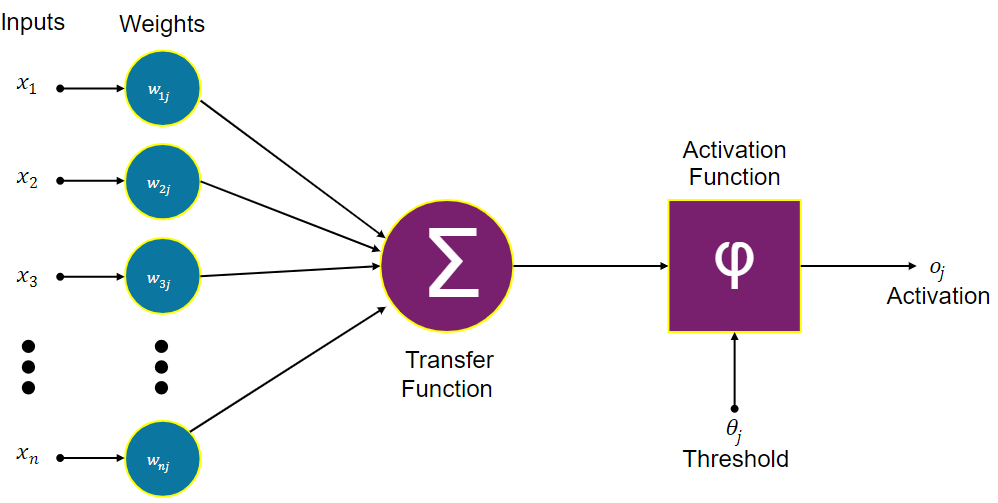
\includegraphics{obrazky-figures/neuron.png}}
    \caption{Umelý neurón \cite{Wikipedia_neuron_2_pokus}.}
    \label{Obraz_2}
\end{figure}

Model na obrázku \ref{Obraz_2} je možné popísať rovnicou \ref{eq:rovnica_neuron}:

\begin{equation}
    {o_j = \varphi\left(\sum_{i=1}^{N} (w_i \cdot x_i) - \theta\right)}
    \label{eq:rovnica_neuron}
\end{equation}

kde $x_i$ sú vstupy neurónu, $w_i$ sú váhy, $\theta$ je prah, $\varphi$ je aktivačná funkcia neurónu a $o_j$ je výstup neurónu.

Veľkosť váh $w_i$ vyjadruje uloženie skúseností do spojení neurónov. Čím je väčšia hodnota, tým je daný vstup dôležitejší. $\vartheta$ označuje prahovú hodnotu aktivácie neurónu \cite{Wikipedia_obrazok}.

Neurónové siete môžu pomocou počítačov vykonávať inteligentné rozhodnutie za pomoci minimálneho zásahu človeka. To preto, lebo dokážu modelovať vzťahy medzi vstupnými a výstupnými dátami, ktoré sú nelineárne a zložité \cite{amazon}. 

Medzi ich výhody patrí schopnosť paralelného spracovania dát. Siete dokážu vykonávať viacej úloh naraz. Nelinearita nám umožňuje modelovať reálne vzťahy medzi vstupom a výstupom. Sú odolné voči chybám, keďže porucha alebo strata jednej, či viacerých buniek nezastaví generovanie výstupu. Rozhoduje na základe pozorovania, vedia sa naučiť rozhodnúť na základe pozorovania vstupných trénovacích dát. Nakoniec majú schopnosť zovšeobecňovať dáta, vedia si odvodiť vzťahy na nevidených dátach. To znamená, že sieť dokáže predpovedať a~správne klasifikovať výstupy \cite{cons_prons_NN}.

K nevýhodám môžeme povedať, že je problematické im dôverovať, pretože nevieme dostatočne presne povedať ako sa sieť dostala k výsledku. Môžu byť aj nepresné ak sme nemali dostatočne natrénovaný model alebo obmedzenú veľkosť dataset. Nakoniec je ťažké zistiť ako kategorizujú dáta alebo vytvárajú predikcie, čiže javia sa nám ako Black box \cite{cons_prons_NN}.

\section{Typy neurónových sietí}
V rámci existencie a vývoja neurónových sietí nám vznikli rôzne architektúry a konfigurácie. Ako to väčšinou v živote býva, každá z nich má svoje pozitívne a negatívne stránky a niektoré sú vhodnejšie na niektoré typy úloh. V nasledujúcom zozname si popíšeme niektoré známe typy neurónových sietí \cite{simplilearn}:
\begin{itemize}
    \item Feed-forward neurónová sieť -- Jedná sa o~najjednoduchšie neurónové siete. Dáta putujú iba jedným smerom. Jej výhody sú rýchlosť a~krátka doba na trénovanie. Väčšina aplikácií v~oblasti rozpoznania vizuálneho vstupu používa tento typ sietí.
    \item Kohonenova samo organizujúca neurónová sieť -- Vektory náhodného vstupu sú vstupom do diskrétnej mapy skladajúcej sa z~neurónov. Vektory sú tiež nazývané rozmery alebo roviny. Aplikácie zahŕňajú použitie k rozpoznaniu vzorov v~dátach, ako je lekárska analýza.
    \item Rekurzívne neurónové siete -- V~tomto type sietí si skrytá vrstva ukladá svoj výstup k~použitiu pre budúcu predpoveď. Výstup sa stáva súčasťou nového vstupu. Aplikácie zahŕňajú konverziu textu na reč.
    \item Konvolučné neurónové siete -- Jedná sa o typ \textit{Feed-forward} sietí. Tento typ sietí berie vstupné dávky po dávkach(batch). To umožňuje sieti pamätať si obraz po častiach. Aplikácie zahŕňajú spracovanie signálov a~obrazov, napríklad rozpoznanie tváre.
\end{itemize}
V~tejto práci budeme výhradne pracovať s~konvolučnými neurónovými sieťami.

\subsection{Aktivačné funkcie}
Aktivačné funkcie sú neoddeliteľnou súčasťou neurónových sietí, ktoré im umožňujú naučiť sa zložité vzory v dátach. Transformujú vstupní signál uzlu v neurónovej sieti na výstupný signál, ktorý sa následne predáva do ďalšej vrstvy. Prinášajú nelinearitu, čo umožňuje schopnosť sieťam naučiť sa zložité mapovanie medzi vstupmi a výstupmi. Správny výber je kľúčový pre trénovanie neurónových sietí, ktoré sa dobre generalizujú a poskytujú presné predikcie. 

Najjednoduchším typom je lineárna aktivačná funkcia. Používajú sa vo výstupnej vrstve pre regresívne úlohy, neposkytujú nelinearitu. Jedná sa o najjednoduchšiu funkciu.

Na výstupe sa používajú dva typy buď funkcia \textit{sigmoid} \cite{aktivacne} alebo \textit{softmax} \cite{aktivacne}. \textit{Sigmoida} vracia hodnoty medzi 0 a 1, užitočná pre binárnu klasifikáciu. \textit{Softmax} je všeobecnejšia sigmoida, používa sa pre viac násobnú klasifikáciu, čiže nebinárne úlohy. Obidve funkcie trpia problémom miznúceho gradientu.

Ako poslednú si spomenieme ReLu funkciu, ktorá sa často používa v neurónových sieťach, konkrétne v skrytých vrstvách. Funkcia vie riešiť problém miznúceho gradientu. Vie prahovať vstupné hodnoty na 0, vracia 0 pre záporné hodnoty a samotný výstup pre kladné hodnoty \cite{aktivacne}.

\subsection{Presnosť a strata}
Presnosť (\textit{accuracy}) a strata (\textit{loss}) sú dôležité metriky pri strojovom učení.

Presnosť sa počíta ako počet správnych predikcií/počet všetkých predikcií, podrobnejšie v podkapitole \ref{metrics}. Presnosť je metóda na meranie výkonnosti klasifikačného modelu. Zvyčajne sa vyjadruje v percentách. Presnosť je počet predpovedí, kde sa predpokladaná hodnota rovná skutočnej hodnote. Je binárna pre konkrétnu vzorku. Presnosť sa zobrazuje v grafe a monitoruje sa počas tréningovej fázy \cite{acc_loss}.

Strata alebo stratová funkcia berie do úvahy pravdepodobnosť alebo neistotu predpovede na základe toho, do akej miery sa predpoveď líši od skutočnej hodnoty. To nám poskytuje presnejší pohľad na výkonnosť modelu \cite{acc_loss}. Existuje niekoľko typov stratových funkcií, ktoré sa používajú v závislosti od úlohy. \textit{Cross-entropy loss} sa používa pri klasifikačných úlohách a hodnotí rozdiel medzi predikovanými a skutočnými kategóriami. \textit{Triplet loss} sa používa pri úlohách rozpoznania tvárí. Snažia sa minimalizovať vzdialenosť medzi pozitívnym párom a maximalizovať medzi negatívnym. \textit{Contrastive loss} používa sa pri párových úlohách, ako je rozpoznanie tváre, snaží sa priblížiť podobné páry a oddialiť nepodobné. Podrobnejšie tieto funkcie rozoberáme v podkapitole \ref{strat_funkcie}. Tieto stratové funkcie umožňujú lepšie prispôsobenie modelu na danú úlohu a poskytujú jasnejší obraz o jeho výkonnosti počas tréningu a testovania.

\section{Konvolučné neurónové siete}
Pred konvolučnými neurónovými \cite{IBM_CNN} sieťami boli používané časovo náročné metódy extrakcie rysov k~identifikácií objektov v~obrazoch. Konvolučné neurónové siete teraz poskytujú jednoduchší prístup ku klasifikácií obrazov a~úlohe rozpoznania objektov, využívajúcich princípy lineárnej algebry, konkrétne násobenie matíc, k~identifikácií vzorov v obraze. Môžu byť výpočtovo náročné a vyžadovať grafické procesory k~trénovaniu modelov.

Konvolučná vrstva je prvou vrstvou konvolučnej siete. Zatiaľ čo konvolučné vrstvy môžu byť nasledované ďalšími konvolučnými vrstvami alebo \textit{pooling} vrstvami, plne prepojená vrstva je finálnou vrstvou. S~každou vrstvou konvolučnej siete rastie zložitosť, identifikuje väčšiu časť obrazu \cite{IBM_CNN}.

\begin{figure}[h]
    \centering
    \scalebox{0.4}{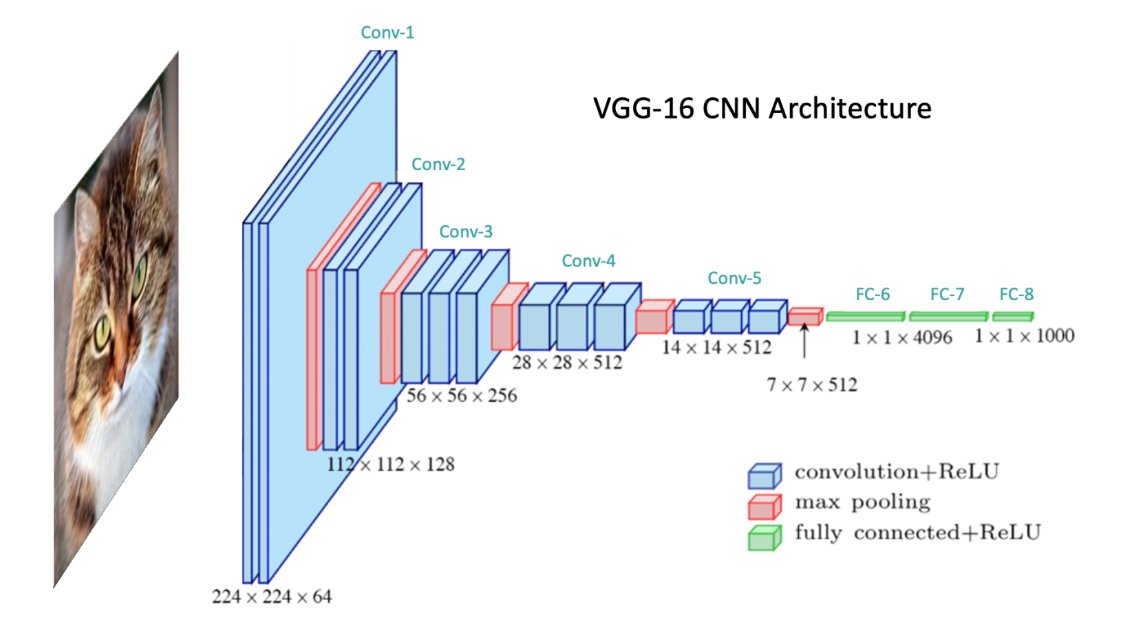
\includegraphics{obrazky-figures/CNN_obrázok.png}}
    \caption{Konvolučná sieť Vgg-16 \cite{learnopencv}.}
    \label{Obraz_4}
\end{figure}

Konvolučné neurónové siete sa odlišujú od ostatných neurónových sietí svojou nadriadenou výkonnosťou pri spracovaní vstupu obrazu alebo zvukových signálov. Majú tri hlavné typy vrstiev:
\begin{itemize}
    \item Konvolučná vrstva
    \item \textit{Pooling} vrstva
    \item Plne prepojená vrstva
\end{itemize}

Na obrázku \ref{Obraz_4} môžeme vidieť ukážku konvolučnej neurónovej siete.

\subsection{Konvolučná vrstva}
Konvolučná vrstva je jadrom stavebného bloku konvolučnej neurónovej siete, a~je to miesto, kde prebieha väčšina výpočtov, vo forme konvolúcie. Vyžaduje niekoľko komponent, a~to vstupné dáta, filter a~príznakovú mapu. Pre každé konvolučné operácie sa aplikuje konvolučná transformácia ReLU (Rectified Linear Unit) na príznakovú mapu, čo do modelu vnáša nelinearitu. Rovnica konvolúcie pre dvoj rozmerné obrázky \cite{convolutional_equation}:
\begin{equation}
    y[i,j] = \sum^{\infty}_{m=-\infty} \sum^{\infty}_{n=-\infty} h[m,n] \cdot x[i - m,j - n]
    \label{eq:rovnica1}
\end{equation}
kde $x$ predstavuje maticu vstupného obrazu, ktorá sa konvoluje s maticou jadra $h$, aby sa vytvorila nová matica $y$, ktorá predstavuje výstupný obraz. Indexy $i$ a $j$ patria obrazovým maticiam, zatiaľ čo indexy $m$ a $n$ patria jadru matice.

\subsection{Pooling vrstva}
\textit{Pooling} vrstvy, sú známe taktiež ako redukcia dimenzie, prevádzajú redukciu dimenzionality, znižujú počet parametrov vstupov. Podobne ako u~konvolučnej vrstve, operácie zlievania prechádzajú filtrom cez celý vstup, ale rozdielom je, že tento filter nemá žiadne váhy. Namiesto toho jadro aplikuje agregačné funkcie na hodnoty v~reaktívnom poli, naplňuje výstupné pole. Existujú dva hlavné typy zlievania \cite{IBM_CNN}:
\begin{itemize}
    \item \textit{Max pooling}: Keď filter prechádza vstupom, vyberá pixel s~maximálnou hodnotou, ktorý zašle do výstupného poľa. Mimochodom, tento prístup je obvykle používaný častejšie než priemerné zlievanie.
    \item \textit{Average pooling}: Keď filter prechádza vstupom, vypočíta priemernú hodnotu v~reaktívnom poli, ktorú zašle do výstupného poľa.
\end{itemize}
Aj keď vo vrstve zlievania dochádza k~strate mnoho informácií, tak má tiež niekoľko výhod pre konvolučné neurónové siete. Pomáha znižovať zložitosť, zlepšovať efektivitu a~obmedzovať riziko nadmernej montáži, \textit{overfitting} \cite{IBM_CNN}.


\subsection{Plne prepojená vrstva}
Názov plno prepojenej vrstvy dobre vystihuje jej povahu. Tak ako sme už spomenuli, hodnoty pixelov vstupného obrazu nie sú priamo prepojené s~výstupnou vrstvou v čiastočne prepojených vrstvách. Viacmennej, v~plno prepojenej vrstve je každý uzol vo výstupnej vrstve priamo pripojený s~uzlom v~prechádzajúcej vrstve. Používa sa na klasifikáciu. Zatiaľ čo konvolučné a~\textit{pooling} vrstvy obvykle používajú funkcie ReLu, plno prepojené vrstvy obvykle využívajú aktivačnú funkciu softmax \cite{softmax} alebo sigmoid k~vhodnej klasifikácií vstupov, produkovanými pravdepodobnosťou od 0 do 1 \cite{IBM_CNN}. 

\section{Architektúra neurónových sietí}

V tejto kapitole sa zameriame na rôzne architektúry neurónových sietí, ktoré zohrávajú kľúčovú úlohu v oblastiach generovania, detekcie a extrakcie vlastností. GAN (\textit{generative adversarial network}) siete slúžia pre generovanie realistických obrázkov, využívajú sa pri tvorbe deepfake. Siamské \cite{siam_doplnok} sú špecifické tým, že obsahujú dve alebo viac identických sietí a určujú ich podobnosť, využitie pri detekcií deepfake. Pre extrakciu vlastností zo snímkov sú často využívané architektúry ako ResNet a Vgg.
Nasledujúce podkapitoly sa podrobnejšie venujú jednotlivým spomenutým architektúram neurónových sietí.

\subsection{Vgg-Net}
Skratka Vgg znamená Visual Geometry Group \cite{vgg-net}, jedná sa o architektúru konvolučnej neurónovej siete. Existujú dve verzie Vgg a~to Vgg-16 a Vgg-19, kde číslovka 16 a~19 označujú počet konvolučných vrstiev. Na obrázku \ref{vgg_arch} môžeme vidieť architektúru siete Vgg16. Táto neurónová sieť sa používa pre identifikáciu objektov. Jedná sa o~populárnu sieť, ktorá vyhrala prvé a~druhé miesto v~súťaži ImageNet Challenge 2014 \cite{vgg-net, simonyan2015deep,imagenet}. Táto architektúra sa dá spoľahlivo použiť na rozpoznávanie tváre, ak je učená na dátovej sade zloženej z tvári ľudí. Nasledujúci obrázok \ref{vgg_arch} zobrazuje architektúru siete Vgg16.

\begin{figure}[H]
    \centering
    \scalebox{0.26}
    {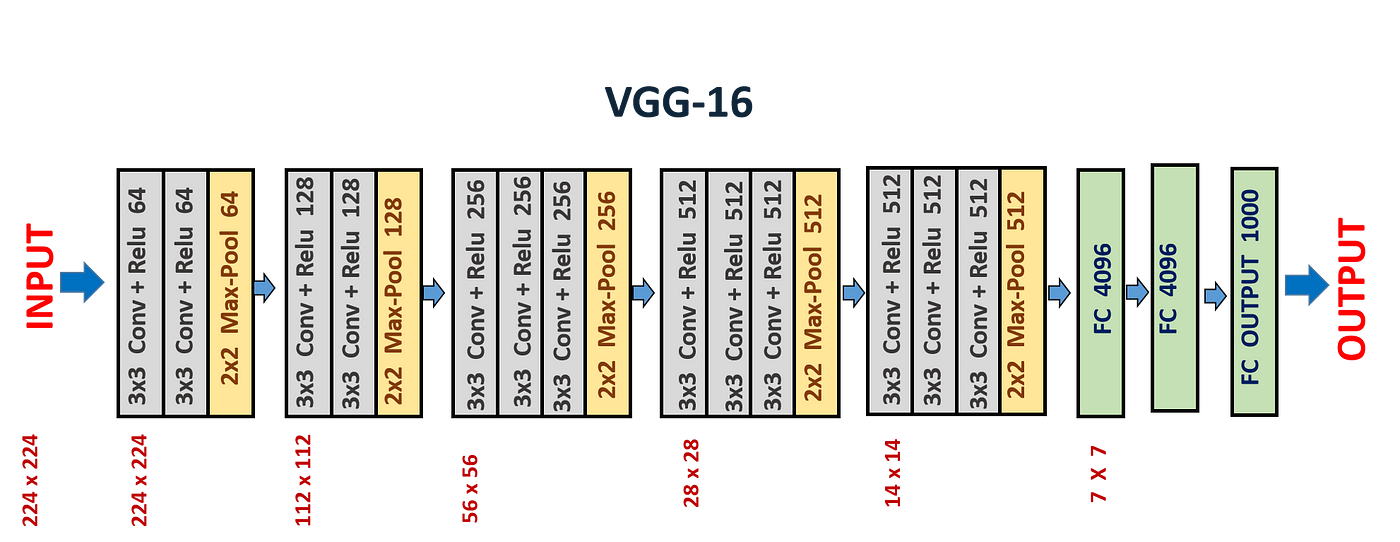
\includegraphics{obrazky-figures/vgg_arch.png}}
    \caption{Architektúra siete Vgg-16 \cite{vgg-net}.}
    \label{vgg_arch}
\end{figure}

\subsection{ResNet}
\textit{Residual Learning} alebo skrátene ResNet architektúra je navrhnutá tak, aby pomohla modelom hlbokého učenia učiť sa rýchlo a efektívne, pomocou zvyškových blokov. Riešia problém degradácie, kedy hlbšia sieť začína fungovať horšie, a taktiež riešia problém miznúceho gradientu, ktorý bráni efektívnemu trénovaniu veľmi hlbokých sietí. Architektúra má rôzne hĺbky s verziami ako 50, 101 alebo 152. Táto sieť našla svoje uplatnenie v aplikáciách hlbokého učenia, najmä počítačového videnia \cite{resnet}. Nasledujúci obrázok \ref{resnet50_arch} zobrazuje architektúru siete ResNet50.

\begin{figure}[H]
    \centering
    \scalebox{0.3}
    {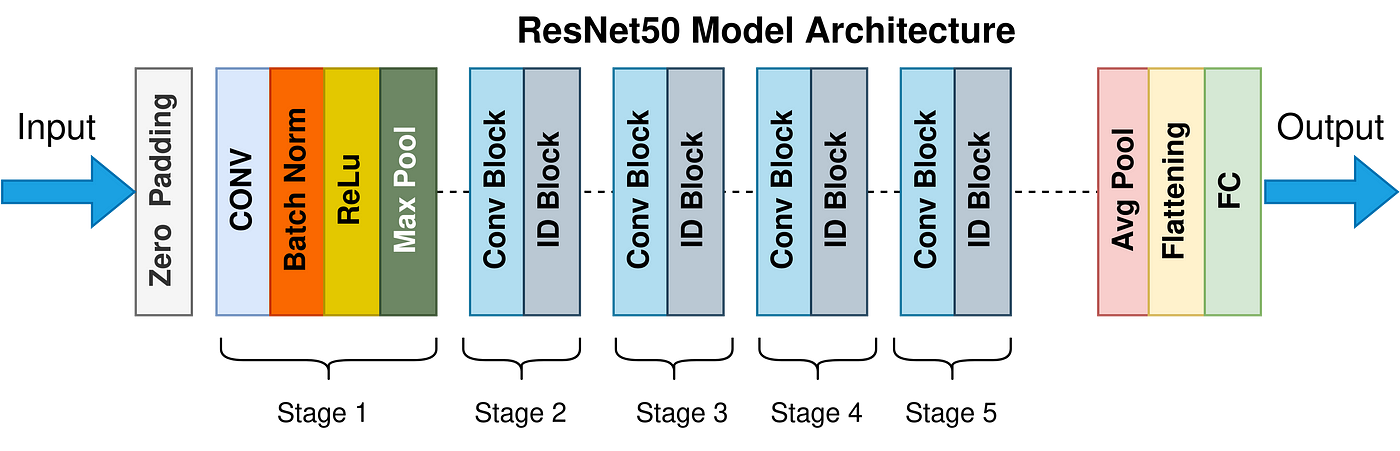
\includegraphics{obrazky-figures/resnet50_image.png}}
    \caption{Architektúra siete ResNet50 \cite{resnet_arch_image}.}
    \label{resnet50_arch}
\end{figure}

\subsection{Siamská neurónová sieť} \label{strat_funkcie}
Siamská neurónová sieť \cite{siam_doplnok} je trieda architektúr neurónových sietí, ktoré obsahujú dve alebo viacero identických sietí. Identické znamená, že majú rovnakú konfiguráciu s~rovnakými parametrami a~váhami. Aktualizácia parametrov počas trénovania je zrkadlená naprieč všetkými sieťami a~používa sa k~nájdeniu podobnosti medzi vstupmi \cite{siam_text}. Nasledujúci obrázok \ref{siamska_arch} znázorňuje štruktúru architektúru siamskej siete. 

\begin{figure}[H]
    \centering
    \scalebox{0.43}
    {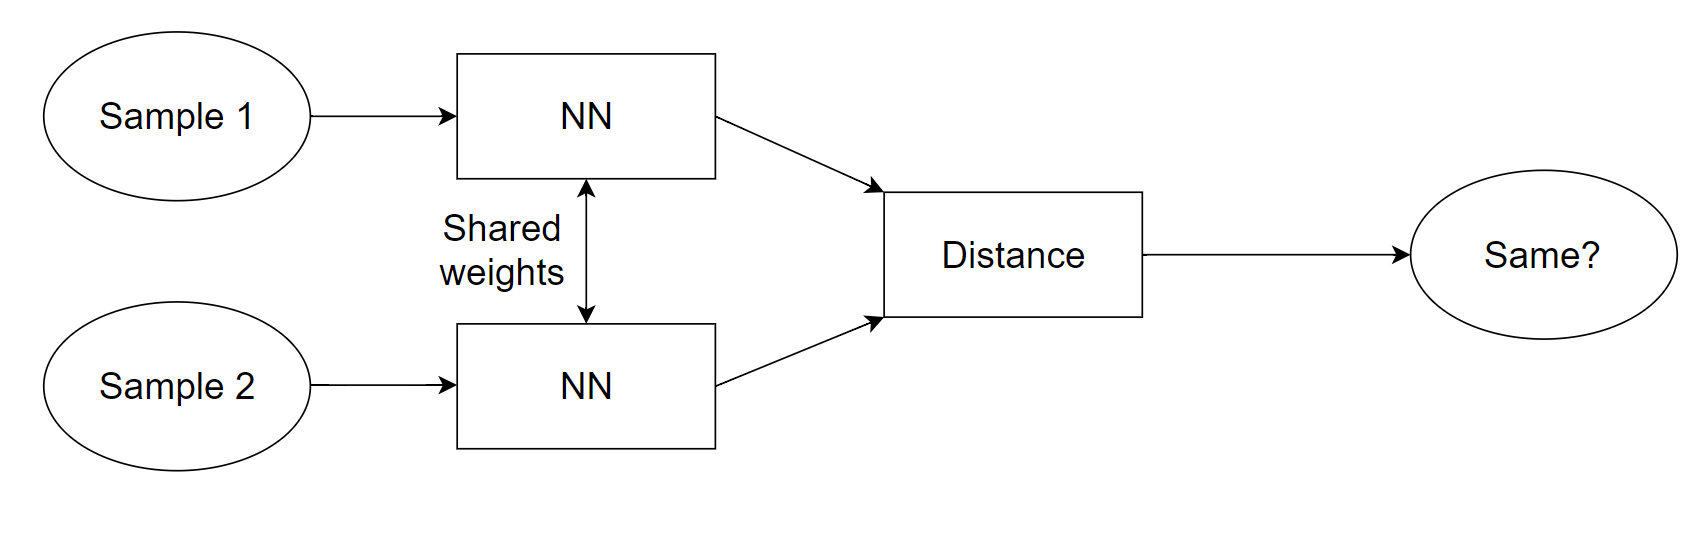
\includegraphics{obrazky-figures/siamska_archt.png}}
    \caption{Architektúra siamskej neurónovej siete. Obrázok vychádza z \cite{zly_siam_snimok}.}
    \label{siamska_arch}
\end{figure}

Siamská sieť dokáže za použitia zopár obrázkov dávať dobré predikcie. Schopnosť učiť sa z~malého množstva dát urobilo siamské siete populárnymi. Táto výhoda je vykompenzovaná dlhším potrebným časom na tréning siete \cite{siam_text}.

Siamské siete našli široké spektrum využitia v~rôznych aplikáciách rozpoznávania obrazu vďaka ich schopnosti efektívne sa učiť reprezentáciu obrazu a~vzájomného porovnávania. V~sfére výskumu rozpoznania ľudskej tváre sú používané k~porovnávaniu dvoch obrazov tváre a~určenia, či patria k~tej istej osobe alebo nie. Môžu byť použité v~sledovaní objektov vo video sekvenciách. Používajú sa k~overovaniu podpisov alebo k~overeniu autentickosti. Kedysi boli využívané aj v~biometrických autentizačných systémov \cite{siam_doplnok}.

Trénovanie siamských sietí môže byť riadené (\textit{supervised}) alebo bez dohľadu (\textit{unsupervised}) \cite{siam_doplnok}. Pri riadenom učení je sieť trénovaná na označených dátach. Pri trénovaní bez dozoru je sieť trénovaná na neoznačených dátach a~musí sa naučiť generovať vlastné označenie na základe vstupných snímkov \cite{siam_doplnok}.

Pri trénovaný je vždy potrebné zvoliť správnu stratovú funkciu. Pri siamských sieťach sa najčastejšie používajú buď \textit{contrastive loss} s~\textit{triplet loss}, každopádne existuje pár scenárov kde \textit{binary cross-entropy} je použiteľná ako napríklad pri úlohách rozpoznania tváre. Stratová funkcia \textit{binary cross-enthropy} má tvar \cite{cross_entro_loss}:

\begin{equation}
L_L = -\frac{1}{N} \sum_{i=1}^{N} \left[ y_i \log(\hat{y}_i) + (1 - y_i) \log(1 - \hat{y}_i) \right]
\end{equation}

kde $\hat{y}_i$ je predpokladaná pravdepodobnosť pre i-tú vzorku, $y_i$ je označenie (\textit{label}) i-tej vzorky. N je celkový počet vzoriek.

\textit{Triplet loss} \cite{losses} používa na vstup 3 obrázky vstupný, pozitívny a negatívny. Funkcia porovnáva vstup s~pozitívnym a~negatívnym obrázkom. Vzdialenosť medzi vstupom k pozitívnemu sa počas trénovania minimalizuje a~vzdialenosť medzi vstupom k~negatívnemu maximalizuje. 

\textit{Contrastive loss} \cite{losses}. je založená na vzdialenosti. Táto stratová funkcia sa snaží pre dva podobné body dávať na výstup nízku euklidovskú vzdialenosť a~pre dva odlišné body veľkú euklidovskú vzdialenosť. Pri tom používa hodnotu \textit{margin}, ktorá udáva minimálnu vzdialenosť, ktorou sa musia nepodobné body držať, takže trestá nepodobné vzorky za to, že sú bližšie než je zadaná hranica. Stratová funkcia \textit{contrastive loss}, využitá v rámci tejto práci, má tvar \cite{7899663}:

\begin{equation}
    \mathcal{L} = (1 - l)D^2 + l \{max(0, m - D)\}^2
    \label{eq:rovnica4}
\end{equation}
kde $l$ je pravdivé binárne označenie snímky, podľa toho či sa jedná o~deepfake $(l = 1)$ alebo originál $(l = 0)$, \textit{margin} > 0 je hranica pre nepodobné páry a $D = || f(Ref) - f(Cand)||_2$ je Euklidovská vzdialenosť medzi vektorom referenčného obrázka $f(Ref)$ a~snímkom pre porovnanie s~referenciou $f(Cand)$ vstupných snímkov modelu. $Ref$ označuje referenčný snímok a $Cand$ kandidátny snímok, čo môže byť potenciálny deepfake. Nepodobné páry prispievajú k~stratovej funkcii iba vtedy, ak je ich vzdialenosť v medziach hodnoty \textit{margin}. Táto stratová funkcia podporuje zhodné páry, aby boli blízko seba vo funkčnom priestore, zatiaľčo odlišné páry sa od seba vzďaľujú \cite{7899663}.

\subsection{GAN architektúra}
GAN architektúra zahŕňa dve neurónové siete: generátor a~diskriminátor, ako je znázornené na Obrázku \ref{Gan_img}. Ak máme súbor skutočných obrázkov $x$ s~distribúciou $p_{data}(x)$, cieľom generátora $G$ je vytvoriť obrázky $G(z)$ podobné skutočným obrázkom $x$ s obrázkami $z$ ako šumovým signálom s distribúciou $p_{z}(z)$. Cieľom diskriminátora $G$ je správne klasifikovať obrázky generované $G$ a skutočné obrázky $x$. Diskriminátor $D$ je trénovaný na zlepšenie svojej klasifikačnej schopnosti, teda maximalizovať $D(x)$, čo predstavuje pravdepodobnosť, že $x$ je skutočný obrázok, a že jeho výstupy budú klasifikované $D$ ako syntetické obrázky, teda minimalizovať $1 - D(G(z))$. Ide o minimaxovú hru medzi dvoma hráčmi $D$ a~$G$, ktorú možno opísať nasledujúcou hodnotovou funkciou \ref{eq:rovnica2}:
\begin{equation}
    {\underset{G}{\min}\, \underset{D}{\max}\, V(D,G) = E_{x~p_{data}(x)}[logD(x)]+E_{z~p_{z}(z)}[log(1-D(G(z)))]}
    \label{eq:rovnica2}
\end{equation}

kde $G$ je generátor, $D$ reprezentuje diskriminátor, $V(D,G)$ je minimax hra medzi generátorom a diskriminátorom, $x$ reprezentuje reálny obrázok s distribúciou $p_{data}(x)$, $z$ je zašumený vstup do generátora, $G(z)$ reprezentuje výstup generátora -- tu sa jedná o nepravý snímok, $D(x)$ je výstup diskriminátora -- čo obsahuje pravdepodobnosť pravosti vstupného obrázky, $D(G(z))$ reprezentuje výstup diskriminátora pri prijatí falošného obrázka z $G(z)$, $p_{data}(x)$ je pravdepodobnostná distribúcia reálneho snímku, $p_{z}(z)$ pravdepodobnostná distribúcia falošného snímku, $E_{x~p_{data}(x)}[logD(x)]$ je priemerná logaritmická pravdepodobnosť $D$, keď je zadaný skutočný obrázok a nakoniec $E_{z~p_{z}(z)}[log(1-D(G(z)))]$ je priemerná logaritmická pravdepodobnosť $D$ pri vstupe vygenerovaného obrázka, čiže falošného \cite{gan_eq1, gan_eq2}.

Po dostatočnom tréningu obidve site zlepšujú svoje schopnosti, teda generátor $G$ je schopný vytvárať obrázky, ktoré sú veľmi podobné skutočným obrázkom, zatiaľ čo diskriminátor $D$ je schopný rozlišovať falošné obrázky od skutočných \cite{NGUYEN2022103525}. Nasledujúci obrázok \ref{Gan_img} znázorňuje architektúru GAN sietí.

\begin{figure}[H]
    \centering
    \scalebox{0.7}{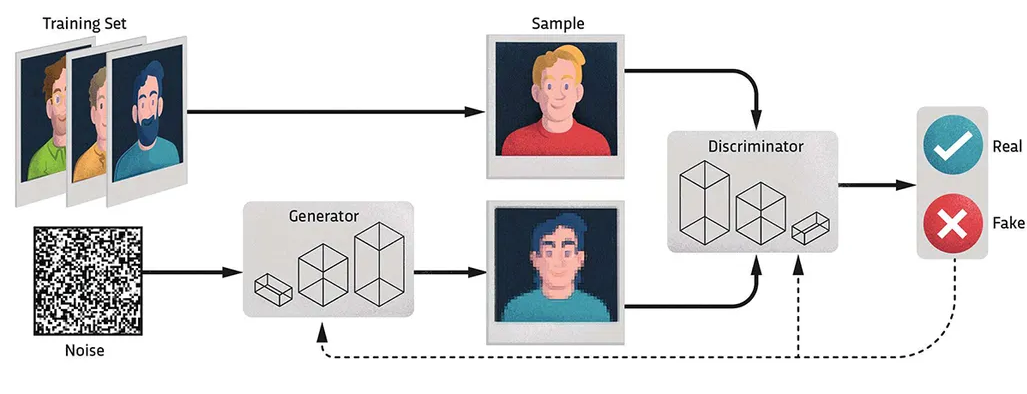
\includegraphics{obrazky-figures/Gan_priklad.png}}
    \caption{Štruktúra GANu \cite{GAN_obrazok2}.}
    \label{Gan_img}
\end{figure}

\chapter{Deepfake tváre}
Myšlienka manipulácie fotografií sa v ľudských mysliach začala tvoriť pri vzniku prvých fotografií, niekedy v~19. storočí. Tieto techniky predovšetkým radi využívajú totalitné režimy \cite{Wikipedia_manipul}. Ich prudký nárast však prišiel so vznikom videí a~vyvrcholil pri pokrokoch umelej inteligencie. Podobne ako bolo zneužívané manipulovanie fotografií v~histórii, tak skoro totožne dopadlo využívanie deepfake technológie. Deepfake môže byť výraznou hrozbou pre spoločnosť vo forme hoaxov v~médiách, politických systémov, jednotlivcov, podnikateľov a~podobne. Z týchto dôvodov je potreba ich detekcie a~regulácie pri zneužívaní \cite{AGARWAL2023223}. Väčšina deepfake algoritmov je založených buď na princípe konvolučných neurónových sietí alebo GAN sietí. Oba tieto prístupy majú kľúčovú úlohu pri tvorbe syntetických obrázkov, tieto obrázky sú zamerané na vizuálnu manipuláciu tváre osôb.

\section{História}
Deepfake označuje špecifický druh synteticky vytvorenej snímky alebo fotografie, ktorý zabezpečuje zmenu tváre osoby alebo osôb za akúkoľvek inú podľa preferencie. Termín deepfake vznikol v~roku 2017 na Reddite po užívateľovi, ktorý tento Reddit spravoval \cite{AGARWAL2023223}. Tento názov je spojenie slov deep learning a~fake. Na začiatku boli pre tvorbu deepfake algoritmov použité neurónové siete \textit{Autoencoders} \cite{autoencoders}. \textit{Autoencoder} je špeciálny typ neurónovej siete, ktorej cieľom je zhodovať sa so vstupom, ktorý bol poskytnutý. Pri deepfakoch sú trénované dva páry autoenkóderoch súčasne a ich parametri sú súčasne zdieľané. Táto stratégia umožňuje bežnému enkodéru nájsť a~naučiť sa podobnosť medzi dvoma sadami tvárí, čo je relatívne jednoduché, pretože tváre obvykle majú podobné rysy, ako sú poloha očí, nosa a úst. Obrázok \ref{Obraz_7} zobrazuje proces vytvárania deepfake, pri ktorom je sada čŕt tváre A spojená s~dekóderom B na rekonštrukciu tváre B z~pôvodnej tváre A. Na obrázku \ref{Obraz_7} môžeme vidieť názornú ukážku použitia enkóderov a dekóderov pri autoenkóderov. Táto verzia sa neskôr vylepšila minimalizujúc množstvo strát. Toto vylepšenie bolo založené na práci Ian Goodfellowa GAN z~roku 2014 \cite{goodfellow2014generative}. Tento pokrok prispel k popularite deepfake technológie ako môžeme vidieť na obrázku \ref{Obraz_1}.

\begin{figure}[h]
    \centering
    \scalebox{0.7}{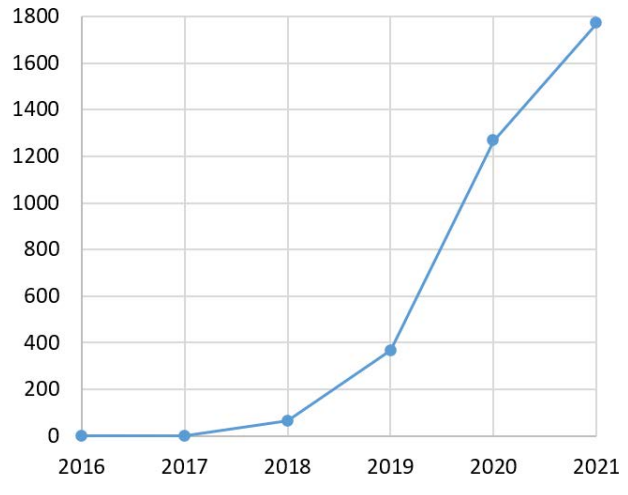
\includegraphics{obrazky-figures/graf_popularity.png}}
    \caption{Graf popularity deepfake v priebehu rokov \cite{NGUYEN2022103525}.}
    \label{Obraz_1}
\end{figure}

V rokoch 2015 a 2016 sa technológia tvorby deepfake zdokonaľovala a~jej prvotný výbuch nastal v~roku 2017, keď sa spoločnosti Nvidia podarilo dosiahnuť významný pokrok v kvalite výstupu GANu \cite{Deepfakes}. V istom roku sa do popredia dostáva už spomínaní reddit server deepfakes, ktorý spopularizoval deepfake technológiu. Tento nárast popularity bol predovšetkým spôsobený propagovaním obsahu pre dospelých, kde tváre protagonistov v jednotlivých scénkach boli nahradené za tváre známych celebrít, predovšetkým ženského pohlavia. Tento reddit bol zrušený v roku 2018 z dôvodu vysokého výskytu nemravného obsahu. Od vtedy prebiehali ďalšie vylepšenia, nové regulácie na sociálnych sieťach, ktoré sa rozhodli, že nechcú na svojich stránkach žiadne deepfake snímky \cite{Deepfakes}. Od tejto chvíle vzniklo veľa \textit{open-source} projektov, ktoré naďalej rozvíjajú túto technológiu.

\begin{figure}[H]
    \centering
    \scalebox{0.9}{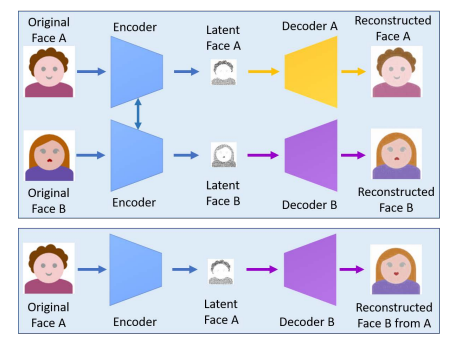
\includegraphics{obrazky-figures/Autoenkoder.png}}
    \caption{Zobrazenie učenia autoenkóderu pri výmene tváre \cite{NGUYEN2022103525}.}
    \label{Obraz_7}
\end{figure}

\section{Problematika deepfake}
Deepfake technológia je v~dnešnej dobe veľmi ľahko dostupná, čo je jeden z najväčších problémov. Tento fakt podporuje aj skutočnosť rýchlo rastúceho počtu podvodných článkov a~videí zachytávajúcich ľudí čo sú pristihnutí pri činnostiach, ktoré nikdy nevykonávali. Ďalší problém vyplýva z~ich sofistikovanosti a~reálnosti. Už dávno sme prekonali dobu kedy tieto pokusy o~podvody boli na prvý okamih jasné, dnes je situácia o~dosť horšia a~algoritmy deepfake technológie dokážu vytvoriť snímky, ktoré nie sú ľahko ľudským okom odlíšiteľné od reálnych. Nasledujúce podkapitoly sa budú venovať problematike pri zmene tváre ľudí a~ich hrozbou pre známych osobností ale aj menej známych a~nakoniec popíšeme potrebu ich detekcie a~či vlastne má význam. Na nasledujúcom obrázku \ref{Deepfae_img} môžeme vidieť príklad tvorby deepfake. 

\begin{figure}[h]
    \centering
    \scalebox{0.6}{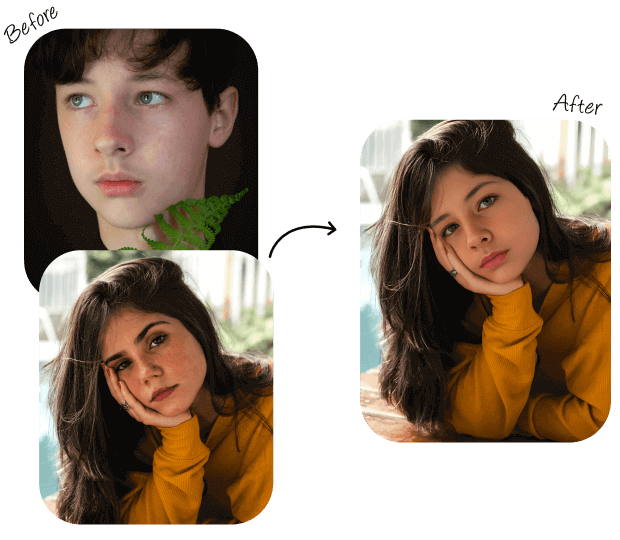
\includegraphics{obrazky-figures/faceswap.png}}
    \caption{Príklad deepfake \cite{deep_obrazok2}.}
    \label{Deepfae_img}
\end{figure}

\section{Zneužívanie deepfake technológie}
Ako už bolo spomínané deepfake je veľmi populárny na stránkach pre dospelých. Väčšina týchto snímkov a~na základe článku \cite{Tension} až 96 \% je vytvorených bez súhlasu protagonistov. Tento žáner reprezentuje videá kde tvár jednej osoby, obvykle ženskej celebrity, je umiestnený na telo druhej. Na podobnom princípe môžu podvodníci využiť vašu fotku a vytvoriť videá alebo obrázky, za cieľom vymáhať z vás peniaze \cite{Distinct}. Na druhú stránku existujú aj humorné účty na sociálnych sieťach, ktoré za súhlasu celebrít, vytvárajú obsah kde si svoju tvár zmenia na celebritu, a~tak zvyšujú popularitu tejto osobnosti \cite{korshunova2017fast}.

Ďalšie odvetvie zneužívania deepfake technológie je v~oblasti politiky. Väčšinou sa jedná o~sfalšovaný prejav politika tak, aby odradili podporovateľov danej osoby. Najlepšia ochrana proti týmto podvodom je prezerať oficiálne profily politikov na sociálnych sieťach, ktoré sú verifikované, či naozaj niečo také vykonal. Takéto výtvory majú potenciál ohroziť demokraciu tak ako sa spomína v článku \cite{deepfake_synthetic_media_reality} a preto je potrebná rýchla detekcia na limitovanie škôd. Jeden z najväčších pokusov o politickú manipuláciu bol pokus Ruskej federácie o vytvorenie deepfake snímku, kde bol vyobrazený Ukrajinský prezident Zelenskyy \cite{skynews}. Nejednalo sa o kvalitný snímok a nebol zásadný problém ho detekovať spravodajskými spoločnosťami \cite{Tension}. Výsledný snímok môžeme vidieť na obrázku \ref{Deepfae_zelenskyy}.

\begin{figure}[h]
    \centering
    \scalebox{0.2}{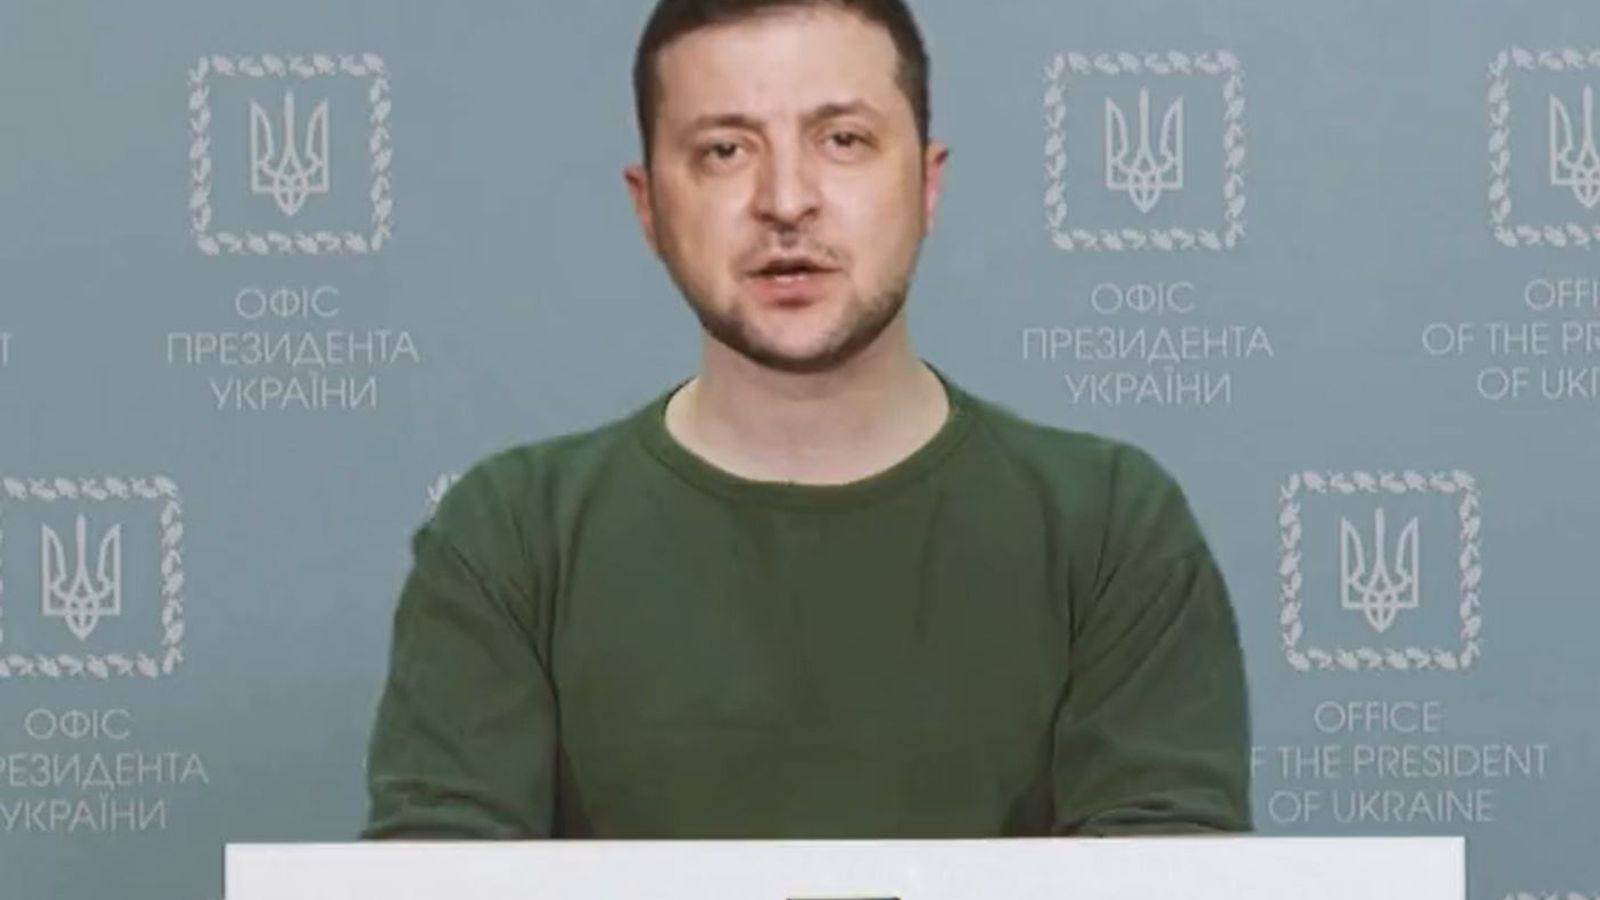
\includegraphics{obrazky-figures/zelensky.jpg}}
    \caption{Zelenskyy deepfake \cite{skynews}.}
    \label{Deepfae_zelenskyy}
\end{figure}

Práve internet a mediálne portály sa snažia byť využité na rozposielanie týchto falošných správ. Novinári už od pradávna bojujú s~hoaxami a~v~priebehu rokov vynašli taktiky ako zabrániť šíreniu falošných správ, avšak tieto praktiky sú prikrátke pri deepfakoch. Obrana voči deepfakom môže stáť nemalý kapitál, preto novinári musia ručne overovať či je daná správa reálna alebo vymyslená. Z tohto dôvodu spoločnosti ako Google alebo Meta vytvorili vlastné projekty, s~ktorými chcú limitovať počet a~rýchlo detekovať deepfake. Do tohto rozsiahleho výskumu je aj zapojených mnoho univerzít, ktoré sa snažia hľadať lepšie a účinnejšie riešenia detekcie deepfake \cite{Deepfake_media_gigants}.

\section{Pozitívne využitie} 
Doteraz boli spomenuté iba negatívne stránky, na ktoré sa žiaľ deepfake technológia prevažne využíva, avšak deepfake má možnosť pozitívne ovplyvniť budúcnosť pri mnohých aplikáciách. V súčasnosti bol deepfake využitý napríklad Davidom Beckhamom, kedy jeho hlas bol menený do rôznych jazykov, aby upozornil čo najväčší dosah ľudí o malárií \cite{deepfake_britannica}. Predpokladá sa, že deepfake technológia by mohla zefektívniť a z atraktívni vzdelanie. Vďaka deepfakom namiesto online kurzov, kde iba niekoho počúvame, by mohli vzniknúť interaktívne kurzy kde by sme mali učiteľa, s~ktorým by sme mohli interagovať a~pýtať sa ho otázky na objasnenie vecí, ktoré nechápeme. Na stávajúcich výukách v školách by napríklad na hodinách dejepisu mohli byť oživené postavy s~dejín, s~ktorými by mohli študenti komunikovať a~názorne ich vidieť pre lepšiu predstavivosť \cite{deepfake_transform_business}. Na školách medicíny by si žiaci mohli lepšie odsimulovať operovanie a komunikáciu s pacientov. Môžeme vytvárať rýchlejšie a~lacnejšie umelecké obrazy, ktoré by boli schopné zrýchliť vývoj softwaru alebo výrobu filmov. Ďalšie odvetvie kde by deepfake vedel výrazne prispieť je virtuálna realita, kde by pomohol naše pomerne realisticky tváre previesť do virtuálnej reality \cite{Deepfake_technology_post_and_neg}.

\section{Deepfake algoritmy}

V nasledujúcej sekcií si bližšie popíšeme dva použité deepfake programy, ktoré sme v práci využili. Tieto dva boli vytvorené pomocou skupiny výskumníkov, čiže sú k nim dostupné aj vedecké články. Ostatné použité programy, boli \textit{open-source} projekty, ktoré neobsahujú žiadne vedecké články. 

\subsection{SimSwap}
SimSwap \cite{simswap_deep} je deepfake program, ktorým cieľom je preniesť identitu zdrojovej tváre na cieľovú tvár pri zachovaní atribútov cieľa, ako je výraz a osvetlenie.

\begin{figure}[h]
    \centering
    \scalebox{0.72}{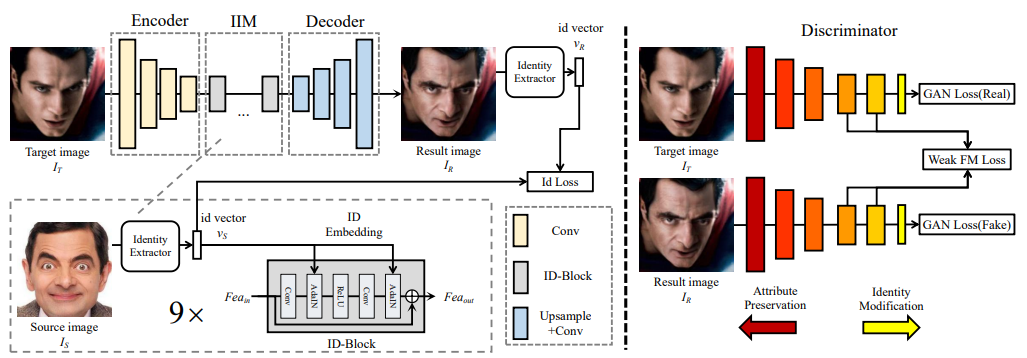
\includegraphics{obrazky-figures/simswap_pipeline.png}}
    \caption{SimSwap pipeline \cite{simswap_deep}.}
    \label{SimSwap_pipeline}
\end{figure}

Implementácie je vytvorená za použitia technológie GAN, konkrétne enkóderu a dekóderu. Medzi nimi je pridaný \textit{Injection Module}(IIM) \cite{simswap_deep}, ktorý zabezpečuje prenos tváre na cieľovú osobu. Enkóder extrahuje tvár osoby $F_{ea_T}$ z cieľového obrázka $I_T$, injekčný model vyextrahuje tvár požadovanej osoby z $I_S$ do $F_{ea_T}$ a dekóder sa postará o vytvorenie výsledného snímku. Ako stratovú funkciu využívajú \textit{Weak Feature Matching Loss} \cite{simswap_deep}, aby sa implicitne zachovali atribúty cieľa. Architektúra je navrhnutá tak, aby sa dala prispôsobiť ľubovoľným identitám. Model bol natrénovaný na datasete VggFace2\footnote{https://paperswithcode.com/dataset/vggface2-1}, ktorý obsahuje širokú škálu tvári v rôznych pozíciách a vekových kategóriách. Využívali snímky ktoré boli väčšie ako $250\times250$ pixelov boli zarovnané a orezané. Autori svoj model popisujú ako revolučný a jeden z najlepších tej doby, ale už nie je najnovší a dnes toto tvrdenie už neplatí \cite{simswap_deep}. 

\subsection{Ghost}
Ghost \cite{ghost_deep} je deepfake program na jednorazové zamieňanie tvárí v obrázkoch a videách, ktorého cieľom je zlepšiť kvalitu a výkon voči moderným architektúram SoTA \cite{sota}. Ghost stavia na architektúre \textit{FaceShifter AEI-Net} \cite{net_faceshifter} s vylepšeniami, ako je stratová funkcia pre oči, algoritmus vyhladzovania tvárovej masky, stabilizačná technika a následné spracovanie v vysokom rozlíšený. Stratová funkcia očí zlepšuje výstup zámeny tváre a vytvára realistickejší výstup. Ďalej sa zameriavajú na straty rekonštrukcie tváre, atribútovej a nepriaznivej straty. Model bol natrénovaný taktiež za pomoci datasetu VggFace2, pričom obrázky boli orezané a zarovnané na rozlíšenie $256\times256$ pixelov. V závere autori prezentujú výsledky, ktorými vykazujú lepšie výkony ako spomínané SoTA architektúry \cite{ghost_deep}.

\begin{figure}[H]
    \centering
    \scalebox{0.68}{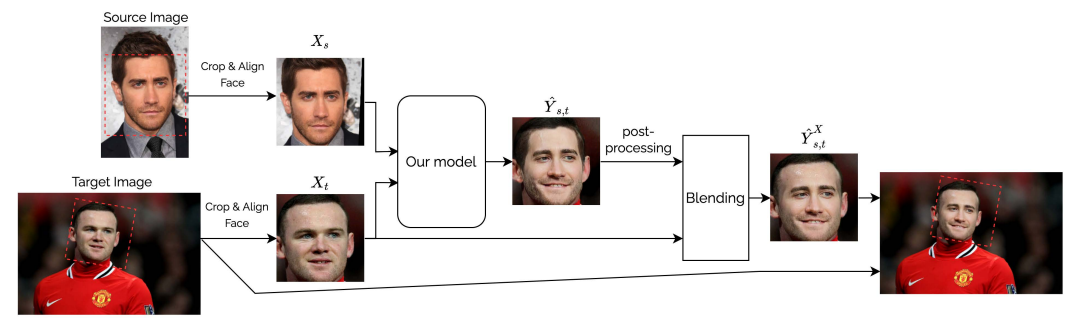
\includegraphics{obrazky-figures/ghost_pipeline.png}}
    \caption{Ghost pipeline \cite{ghost_deep}.}
    \label{Ghost_pipeline}
\end{figure}

Ghost pracuje s orezanými tvárami, preto najskôr pred výmenou tváre musíme orezať zdrojový a cieľový snímok. Po prevedený výmeny tváre sa výsledok vloží do pôvodného cieľového obrázka. Hlavný problém nastáva pri zachovaný atribútov z $X_t$ na $\hat{Y}_{s,t}$, pretože nie sú úplne rovnaké. Preto ak by sme vložili $\hat{Y}_{s,t}$ priamo späť do cieľového obrázka, boli by viditelné okraje ako môžeme vidieť na obrázku \ref{Ghost_smooth}. Riešeným je využiť vyhladzovaciu masku.  Všeobecný postup riešenia Ghost zobrazený na obrázku \ref{Ghost_pipeline} \cite{ghost_deep}:
\begin{itemize}
    \item Detekcia a orezanie tvárí zo zdrojového a cieľového obrázku pomocou detektora tváre. Nech $X_s$ a $X_t$ sú orezané obrázky.
    \item Aplikácia Ghost modelu na $X_s$ a $X_t$ na získanie výsledku $\hat{Y}_{s,t}$.
    \item Zmiešanie $\hat{Y}_{s,t}$ a $X_t$ na získanie finálnej tváre $\hat{Y}^X_{s,t}$
    \item Vloženie výsledku $\hat{Y}^X_{s,t}$ späť do cieľového snímku.
\end{itemize}

\begin{figure}[h]
    \centering
    \scalebox{0.7}{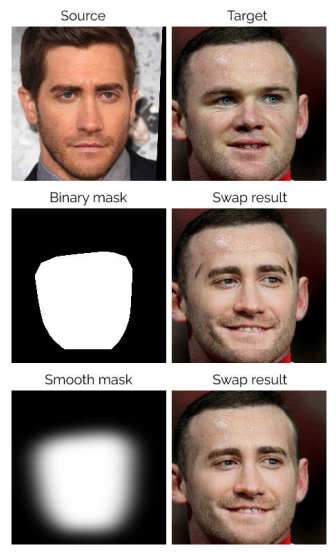
\includegraphics{obrazky-figures/ghost_maska.png}}
    \caption{Ghost maska \cite{ghost_deep}.}
    \label{Ghost_smooth}
\end{figure}

\section{Princíp detekcie deepfake}
Detekcia deepfake je dôležitý výskum, ktorý pomáha nájsť a~zabrániť škodám, ktoré môže vzniknúť z falošných videí a obrázkov. Pri detekovaní deepfake sa experti snažia nájsť stopy, chyby a rozdiely vo videu, ktoré by naznačili upravený súbor. Hľadajú sa divné vzory, rozdiely v~osvetlení alebo čokoľvek neprirodzené. Naviac za pomoci rôznych programov môžeme pozorovať rozdiely v~žmurkaní alebo pohybu tváre osôb. Ďalší spôsob je zaviesť metódy hlbokého učenia, ktoré dokážu zachytiť drobné detaily ľahko nepovšimnuté ľudskými zmyslami. V nasledujúcej časti si bližšie priblížime techniky odhaľovania deepfake \cite{Deepdetect}.

\subsection{Analýza tváre}
Analýza tváre detekuje deepfake prostredníctvom skúmania rysov tváre a~výrazov, identifikujúce nekonzistenciu a~nepravidelnosť. Tento proces využíva počítačového videnia a~strojového učenia k~rozlíšeniu medzi skutočným a~zmanipulovanými tvarmi. Znaky tváre ako oči, nos, ústa a~obočie sú veľmi dôležité pre detekciu deepfake pri analýze tváre. Algoritmy detekcie tieto znaky tváre analyzujú, aby našli rozdiel naznačujúci zmanipulovaný snímok, deepfake snímky často obsahujú v~oblasti tváre rôzne anomálie a nedokonalosti. Techniky detekujú príznaky ako rozmazané hrany, spomínané osvetlenie a nesúlad v textúrach tváre. Strojové učenie zlepšilo analýzu tváre pre detekciu, že analyzuje artefakty a rozlišuje medzi autentickou a~zmanipulovanou tvárou. Hlboké učenie môže detekovať manipulácia prostredníctvom analýzy jemných vizuálnych signálov v~rozsiahlych dátových sadách s~veľkou presnosťou \cite{Deepdetect}.

\subsection{Forenzná analýza}
Forenzná analýza detekuje deepfake skúmaním digitálnych dôkazov a~identifikáciu manipulácie. Táto metóda odhaľuje skryté stopy zanechané behom vytvárania alebo úprav deepfake. Forenzná analýza je zásadná pre rozlíšenie autentickosti a detekcii deepfake. Forenzná analýza detekuje obsah deepfake a~skúma metadáta. Metadáta ukazujú históriu súboru. Analýza metadát rozlišuje autentické od zmanipulovaných, zatiaľ čo forenzná analýza identifikuje nezrovnalosti v obsahu deepfake. Analýza nezrovnalostí v deepfakoch zahŕňa skúmanie zarovnania, osvetlenia, tieňov a~odrazov k~detekcii zmanipulovaných rôznych tvárí na telách \cite{Deepdetect}.

\subsection{Analýza synchronizácie pier}
Analýza synchronizácie pier detekuje deepfake, ktoré manipulujú alebo syntetizujú reč. Prostredníctvom skúmania synchronizácie pohybu pier a~zvukov môžu vedci identifikovať nesúlad naznačujúci deepfake. Analýza pier je zásadná pre odhalenie deepfake. Jedná z~variant je sledovať a študovať pohyb pier vo videu. Počítačové videnie detekuje a~sleduje polohu, tvár a~pohyb pier. Potom sa porovná s~audiom, aby sa vyhodnotila synchronizácia. Analýza skúma vizuálne signály prirodzenej reči. Analýza synchronizácie pier kombinovaná s~forenznou a tvárovou alebo audio analýzou zlepšuje celkovú pravdepodobnosť detekovať deepfake \cite{Deepdetect}.

\subsection{Analýza metadát}
Analýza metadát je kľúčová pre identifikáciu deepfake prostredníctvom posudzovania metadát mediálnych súborov. Metadáta poskytujú podrobnosti o~pôvode, úpravách a~histórii súboru, ponúkajú užitočné informácie o~autentickosti a~možnej manipulácií. Analýza metadát môže odhaliť deepfake skúmaním časovej značky. Časové značky ukazujú aktivitu súboru. Nekonzistentné časové značky zvyšujú podozrenie na možný deepfake. Dôležité je tiež skúmať informácie o~zariadeniach v~metadátach. Digitálne zariadenia ukladajú metadáta, ktoré môžu overiť autentickosť. Tvorcovia deepfake môžu naraziť na problémy s~replikáciou presných metadát fotoaparátov, čo vedie k~nezrovnalostiam. Analýza metadát taktiež môže zahŕňať skúmanie digitálnych podpisov a~vodoznakov. Skúmaním vlastníctva deepfake súboru môžeme ukázať či sa jedná o legitímny obsah. Ďalšou technikou detekcie deepfake je použitie rekurzívnych neurónových sietí navrhnutých k~analýze časových informáciám vo videách. To napomáha identifikovať manipulované znaky, ako sú žmurkanie alebo problémy so synchronizáciou pier. GANy sú taktiež používané v~deepfake detekcií. Sú trénované, aby sme dostávali realistický výstup pomocou generátoru, pričom trénujeme aj diskriminátor, ktorý umožňuje detekovať deepfake \cite{Deepdetect}. 

\section{Detekcia deepfake}
K~využitiu strojového učenia pri detekcií deepfake treba kvalitné rozsiahle dátové sady. Dátové sady obsahujú autentické, tak aj deepfake súbory, poctivo vybrané, aby poskytovali rôznorodé scenáre pre efektívnu detekciu manipulovaného obsahu. Konvolučné neurónové siete sú populárnou metódou pre analýzu vizuálnych dát, z pravidla pri rozpoznávaný obrazových dát. Ich trénovanie na dátových sadách deepfake im umožňuje rozoznať vzory, ktoré odlišujú skutočný obsah od zmanipulovaného \cite{Deepdetect}. V nasledujúcej časti si popíšeme 3 algoritmy na detekciu deepfake. V nasledujúcej časti si popíšeme zopár existujúcich riešení detekcie deepfake.

\subsection{Detekcia za použitia konvolučných sietí}
V tomto článku autori riešia všeobecne problém a rozvoj manipulácie tváre za posledné roky. Článok sa zaoberá detekciou manipulácie tváre vo videách za použitia state-of-art metód. Ponúkajú riešenie problematiky pomocou konvolučných neurónových sietí, konkrétne prezentujú využitie siamskej siete a trénovanie za použitia \textit{end-to-end} prístupu. Do trénovania pomocou \textit{end-to-end} prístupu posielajú na vstup tvár a sieť pošle výsledok na výstup. Ako stratovú funkciu využívajú \textit{LogLoss} funkciu, inak prezívanú aj \textit{binary cross-entropy}, v tvare \cite{cnn_detekcia1}:

\begin{equation}
L_L = -\frac{1}{N} \sum_{i=1}^{N} \left[ y_i \log(S(\hat{y}_i)) + (1 - y_i) \log(1 - S(\hat{y}_i)) \right]
\end{equation}

kde $\hat{y}_i$ predstavuje výstup i-tej tváre, $y_i$ patrí {0,1} štítku (\textit{label}) tváre. 0 označuje reálne tváre a 1 označuje zmanipulované snímky. N je celkový počet tvárí použitých na trénovanie a $S(x)$ je Sigmoidná funkcia.

Pri trénovaný siamskej siete bola využitá stratová funkcia \textit{triplet loss} v tvare \cite{cnn_detekcia1}:

\begin{equation}
L_T = \max(0, \mu + \delta_+ - \delta_-)
\end{equation}

kde $\delta_+ = |f(I_a) - f(I_p)|_2$, $\delta_- = |f(I_a) - f(I_n)|_2$ a $\mu$ je striktne pozitívny okraj. V tomto prípade $I_a$ je kotva (\textit{anchor}), reálny snímok, $I_p$ je pozitívny snímok patriaci rovnakej triede ako $I_a$, ďalší reálny a $I_n$ je negatívny snímok patriaci inej triede ako $I_a$, zmanipulovaný snímok \cite{cnn_detekcia1}.

V rámci práce využívajú viacero architektúr neurónových sietí ako napríklad EfficientNetB4 alebo XceptionNet. Prezentujú výsledky na dvoch verejne dostupných datasetoch s viac ako 119 000 videami. Podrobnejšie informácie sú vo vedeckom článku \cite{cnn_detekcia1}.

\subsection{Detekcia za použitia autoenkóderu}
V tomto článku autori predstavujú riešenie detekcie zmanipulovaných obrázkov za použitia autoenkóderu s názvom MARLIN. MARLIN sa zameriava na rôzne úlohy analýzy tváre, ako sú rozpoznávanie vlastností tváre, rozpoznávanie výrazov tváre, detekcia deepfake a synchronizácia pier. Na nasledujúcom obrázku \ref{Marlin_pipeline} si bližšie popíšeme jednotlivé fázy MARLINu:

\begin{figure}[h]
    \centering
    \scalebox{0.44}{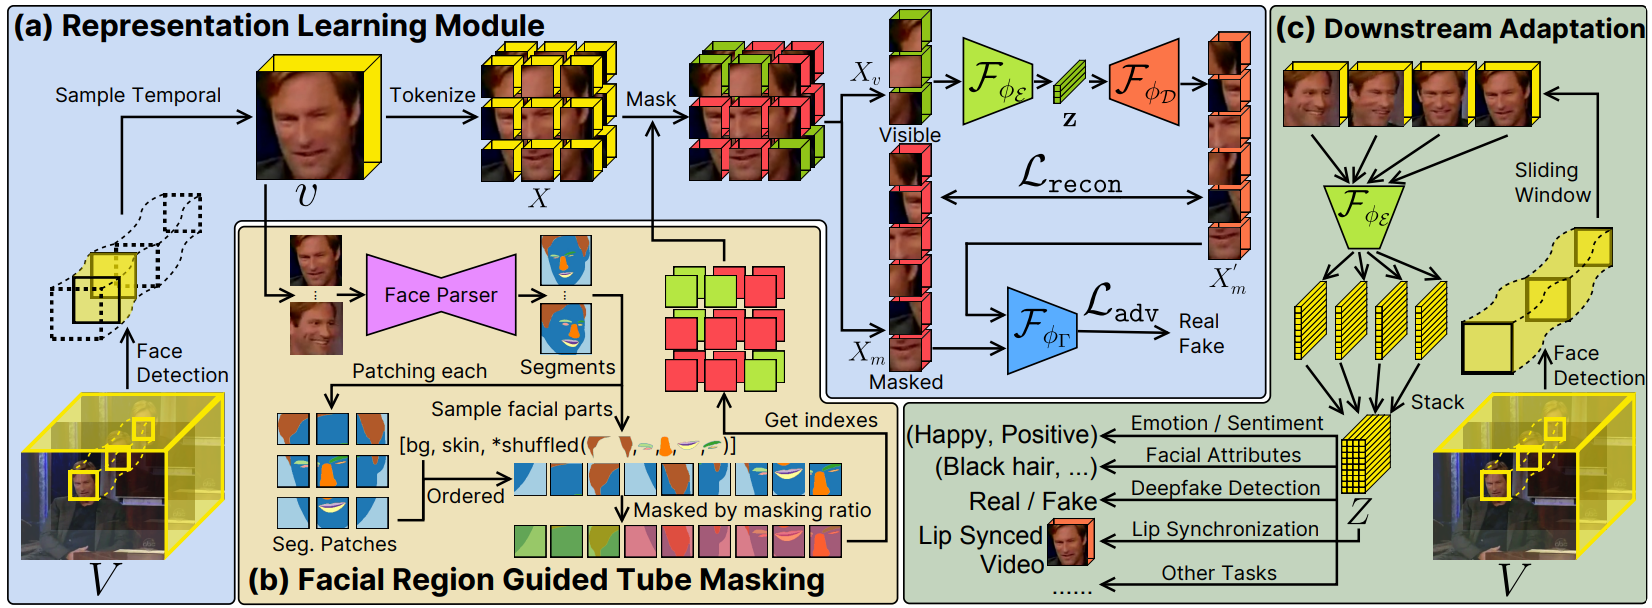
\includegraphics{obrazky-figures/Marlin.png}}
    \caption{Architektonický prehľad MARLIN \cite{cnn_detekcia2}.}
    \label{Marlin_pipeline}
\end{figure}

MARLIN pozostáva hlavne z modulu \textit{Representation Learning Module} (a), \textit{Facial Region guided Tube Masking} (b) a Downstream Adaptation (c). (a) Reprezentačný modul: MARLIN sa učí tvár reprezentovať z neoznačených dát. Jedná sa o  \textit{self-supervised} učenie, zvýraznené modrou farbou. (b) Vedenie podľa oblasti tváre: Pomocou maskovacej trubice vedenej v oblasti tváre (zvýraznené žltou) získava MARLIN dočasné časopriestorové poznatky, ktoré následne využíva na zvýšenie výkonu. Stratégia maskovania trubice vnáša do procesu znalosti domény. (c) Prispôsobenie prúdu: Na prispôsobenie prúdu sa pri špecifických úlohách tváre využíva linéarne snímanie (LP) a jemné ladenie (FT), ktoré sa starajú o robustnosť, generalizáciu a o presnosť načítaného prvku, zvýraznenie zelenou farbou.

Použité dáta pre trénovanie pochádzajú z verejne dostupných videí na YouTube a datasetov ako LFW, CelebA, Vgg-FACE a ďalších. Pre vyhodnotenie výsledkov pri detekcií deepfaku využili dataset FaceForensic++. Podrobnejšie informácie sú vo vedeckom článku \cite{cnn_detekcia2}.

\chapter{Algoritmy pre rozpoznanie tváre}
Oblasť skúmania tváre je jednou z~najrozšírenejších oblastí v~počítačovom videní. Rozpoznanie tváre je spôsob identifikácie alebo potvrdenia identity jednotlivca pomocou jeho tváre \cite{kaspersky}. Systémy rozpoznania tváre slúžia k~identifikácií ľudí na fotografiách, videách alebo v~reálnom čase. Všetky tieto funkcionality sú vytvorené pomocou algoritmov na rozpoznanie tváre, ktoré sú vyvíjané od roku 1960 a~od tej doby ich vzniklo mnoho rôznych variant \cite{face_rec_algo}.

V~tejto kapitole priblížime pozadie za algoritmami a~metódami pre rozpoznanie tváre ich architektúru a~problematiku, ktorá musí byť prekonaná pri detekciách tváre osoby zo snímky.

\section{Architektúra systému}
Vstupom do systému rozpoznávania je vždy fotografia alebo video. Výstupom je identita, vektor alebo boolovská hodnota áno/nie, závisí podľa danej úlohy. Existujú prístupy, ktoré definujú systém rozpoznania ako trojstupňový proces.
\begin{figure}[h]
    \centering
    \scalebox{0.5}{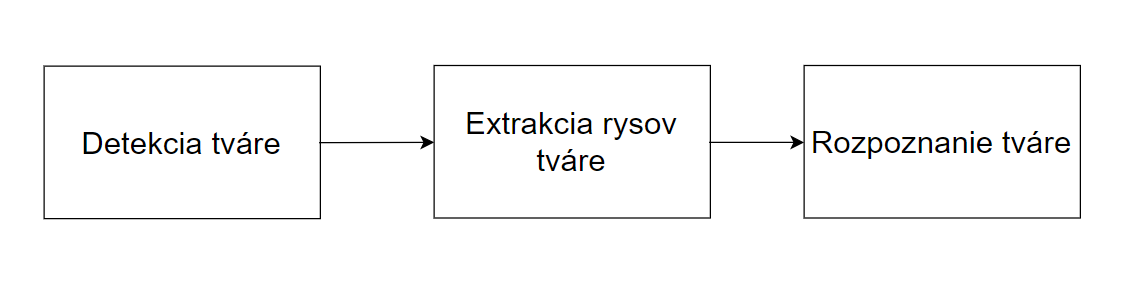
\includegraphics{obrazky-figures/Architektura_face_rec.png}}
    \caption{Obecný systém rozpoznania tváre \cite{face_rec_algo}.}
    \label{Obraz_5}
\end{figure}
Z tohoto hľadiska by bolo možné vykonať fázu detekcie tváre a~extrakcie rysov súčasne. Detekcia tváre je definovaná ako proces extrakcie tvár zo scén. Systém tak pozitívne identifikuje určitú oblasť obrazu ako tvár. Tento prístup má mnoho aplikácií, ako je sledovanie tváre, odhad polohy alebo kompresia. 

Existuje niekoľko kategórií pre algoritmy rozpoznania tváre. Prvý je založený na geometrickom prístupe. Táto kategória zahŕňa algoritmy, ktoré analyzujú rysy tváre a ich geometrické vzťahy. Môžu extrahovať parametre ako vzdialenosť medzi očami, nosom a ústami alebo uhly medzi nimi. 
Ďalšia kategória je na základe holistických modelov, kde sa na tvár dívame ako na celok. Namiesto toho, aby sa zameriavali na jednotlivé rysy, tieto algoritmy skúmajú celkovú štruktúru tváre. V tomto prípade sú používane konvolučné neurónové siete, aby sa naučili reprezentáciu tváre \cite{cat_face1,cat_face2}.

Ďalším krokom môže byť extrakcia rysov, kde získavame relevantné tvarové rysy z dát. Tieto rysy môžu obsahovať relevantné údaje o~tvári ako časti tváre, uhly alebo rozmery ako napríklad rozostup očí, najčastejšie sa snaží ako prvé vyhľadať ľudské oči, pretože sa jedná o jeden z~najjednoduchších rysov pri detekcií. Potom sa snaží detekovať charakteristické body tváre, ako sú obočie, ústa, nos \cite{face_rec_algo,face_detect}. 

Najčastejšie používaný prístup namiesto extrakcií rysov je \textit{Face embedding}. Táto metodika reprezentuje tvár ako číselné vektory, zachytávajúce detaily tváre. \textit{Face embedding} je numerická reprezentácia tváre v nízkorozmernom priestore, ktorá umožňuje porovnávať a určovať podobnosť medzi tvárami na základe ich vzdialeností v tomto priestore. \cite{face_embed}.

\section{Detekcia tváre}
V~niektorých prípadoch sa dá detekcia tváre preskočiť. Príkladom môže byť databáza kriminálnikov, kde orgány vyšetrovania ukladajú tváre ľudí s kriminálnym záznamom. Avšak bežné vstupné obrazy systémov počítačového videnia nie sú tak vhodné. Môžu obsahovať mnoho položiek alebo tvárí. V~týchto prípadoch je detekcia tváre povinná. Je tiež nevyhnutná, ak chceme vyvinúť automatizovaný systém sledovania tváre. Preto je rozumné predpokladať, že detekcia tváre je súčasťou širšieho problému rozpoznania tváre \cite{face_rec_algo}.

Detekcia tváre je ovplyvňovaná niekoľkými výzvami ako napríklad \cite{face_rec_algo, AGARWAL2023223}:
\begin{itemize}
    \item Starnutie -- Tvár sa mení s~časom, čo môže mať dopad na algoritmy pre rozpoznanie tváre. Využívajú sa spojené auto-enkodéry pre starnutie a~odstarnutie a skúma ich vplyv na rôzne vekové skupiny.
    \item Termálne obrazy -- Pre rozpoznanie tváre z~termálnych obrazov je hlavné nájsť vhodnú techniku pre extrakciu rysov z~tváre. Vo výskumu sa využívajú Gaborove systémy nízkeho rozlíšenia.
    \item Zakrytie čŕt -- Prítomnosť prvkov ako brady, okuliare alebo klobúk zavádza vysokú variabilitu. Tváre môžu byť tiež čiastočne zakryté objektmi alebo inými tvárami.
    \item Variácia postoja -- Ideálny scenár pre detekciu tváre by bol taký, v~ktorom by boli zahrnuté len čelné obrazy. Ale, ako je uvedené, to je všeobecne veľmi nepravdepodobné v nekontrolovaných podmienkach. Navyše výkon algoritmov detekcie tváre dramaticky klesá pri veľkých variáciách postoja. Je to závažný výskumný problém. Variácia postoja môže nastať v dôsledku pohybov subjektu alebo uhlu kamery.
    \item Výraz tváre -- Črty tváre sa tiež veľmi menia kvôli rôznym výrazom tváre.
    \item Podmienky snímania -- Rôzne kamery a podmienky okolia môžu ovplyvniť kvalitu obrazu, ovplyvňujúc vzhľad tváre.
\end{itemize}

\section{Architektúra štruktúry 
systému rozpoznania tváre}
Detekcia tváre je koncept, ktorý zahŕňa mnoho podproblémov. Niektoré systémy detekujú a~lokalizujú súčasne, iné najskôr vykonajú rutinnú detekciu a~potom, ak je výsledok pozitívny, sa pokúsia lokalizovať tvár. Potom môže byť potrebných niekoľko sledovacích algoritmov - ukážka obrázka \ref{Obraz_6}.
\begin{figure}[h]
    \centering
    \scalebox{0.6}{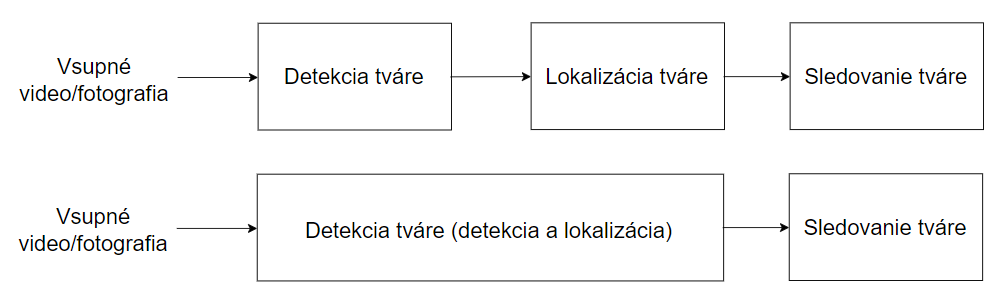
\includegraphics{obrazky-figures/Architektura_face_rec_detekcia.png}}
    \caption{Architektúra detekcie systémov rozpoznania tváre \cite{face_rec_algo}.}
    \label{Obraz_6}
\end{figure}
Algoritmy detekcie tváre zvyčajne zdieľajú spoločné kroky. Po prvé, sa vykoná redukcia dimenzie dát, aby sa dosiahla prijateľná doba odpovede. Niektoré predspracovania môžu byť vykonané aj na prispôsobenie vstupného obrazu predpokladom algoritmu. Potom niektoré algoritmy analyzujú obraz taký, aký je, a iné sa snažia extrahovať určité relevantné oblasti tváre. Ďalšia fáza zvyčajne zahŕňa extrakciu tvárových čŕt alebo meraní. Tieto budú následne vážené, vyhodnotené alebo porovnané, aby sa rozhodlo, či je prítomná tvár a kde sa nachádza. Nakoniec niektoré algoritmy majú rutinu učenia a zahŕňajú nové údaje do svojich modelov. Detekcia tváre je teda problém s dvomi triedami, kde musíme rozhodnúť, či je na obrázku tvár alebo nie. Sledovanie tváre sa rieši najmä vtedy, keď na vstup príde video. V tejto práci budeme pracovať iba so snímkami tváre \cite{face_rec_algo}.

\section{Metódy detekcie tváre}
Nie je ľahké poskytnúť všeobecnú metódu detekcie tváre. Neexistuje všeobecne akceptované kritérium pre všetky skupiny. Obvykle sa miešajú a~prekrývajú. V~tejto časti budú predstavené rôzne metódy detekcie tváre.
\begin{itemize}
    \item Algoritmus Viola-Jones \cite{viola_jones} -- Táto metóda je založená na tréningu modelu, ktorý rozumie čo je a~čo nie je tvár. Jedná sa o~populárny \textit{framework} pre rozpoznávanie tváre v reálnom čase, má problémy s~identifikáciou tváre, ktorá je zakrytá alebo natočená do strany.
    \item Detekcia tváre založená na znalostiach -- Táto metóda spolieha na sadu pravidiel vyvinutých ľuďmi podľa našich znalostí. Vieme, že tvár musí obsahovať oči, nos a~ústa v určitej vzdialenosti a~polohách navzájom. Problém metódy je vytvoriť vhodnú a~jasnú sadu pravidiel. Treba nájsť stred medzi všeobecnými a~veľmi špecifickými \cite{face_rec_med}.
    \item Založené na vzhľade -- Táto metóda používa statickú analýzu a~strojové učenie k~nalezeniu relevantných charakteristík obrazu tváre.
    \item Založené na konvolučných neurónových sietí -- Sieť sa učí rozpoznať a~klasifikovať tvár osoby \cite{face_rec_med2,face_detect}. V nasledujúcej časti si popíšeme niektoré takéto riešenia.
\end{itemize}

\subsection{YOLO (You Only Look Once)}
Jedná sa o inovatívny prístup na detekciu a lokalizáciu objektov, ktorý spracúva obrazy v reálnom čase za použitia konvolučnej neurónovej sieti. Rozdeľuje vstupný obraz na mriežku buniek a predikuje ohraničujúce rámy rôznej veľkosti a tvaru, ktoré slúžia ako referencia predikcie. Toto ohraničenie sa nazýva kotvou, ktoré sú preddefinované ohraničujúce rámy a práve kotvy pomáhajú YOLO generalizovať detekcie pre rôzne typy objektov a mierky. Ohraničujúce rámy sú predikované pomocou konvolučných sietí \textit{region proposal neural networks} (RPN) \cite{rpn}. Pomáhajú zvýšiť presnosť detekcie. Práve vďaka svojej flexibilite a efektívnosti sa dostal do širokej škály odvetví aplikácií počítačového videnia \cite{yolo,yolo_stranka}.

\begin{figure}[h]
    \centering
    \scalebox{0.6}{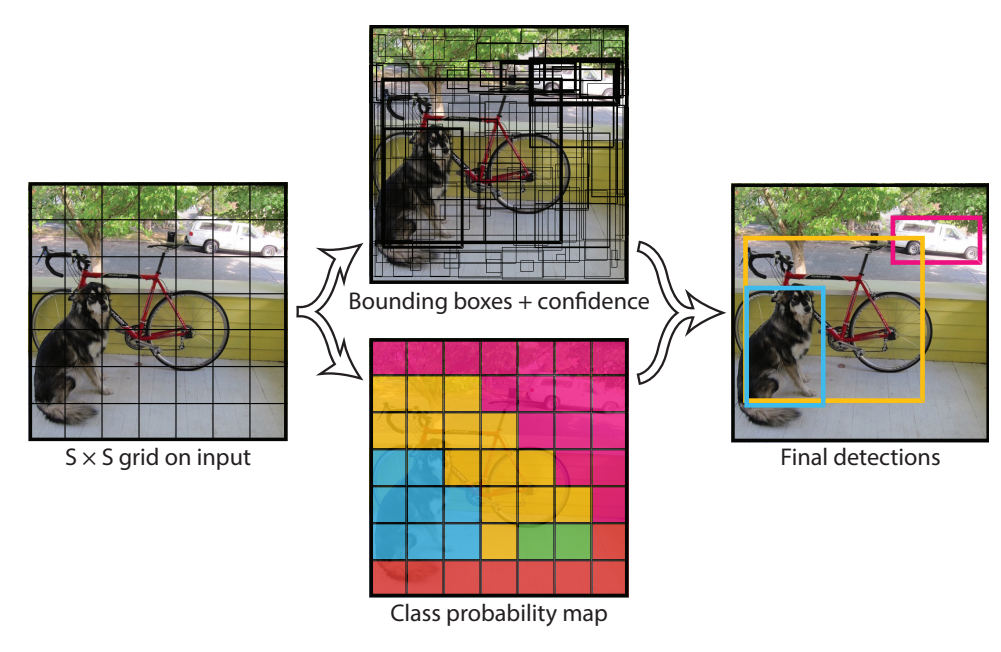
\includegraphics{obrazky-figures/YOLO-arch.png}}
    \caption{Princíp YOLO modelu \cite{yolo}.}
    \label{yolo}
\end{figure}

Na obrázku \ref{yolo} môžeme vidieť rozdelenie obrázku do mriežok. Ďalej odhad rámov/kotiev, na ich základe sa určí odhad o aký objekt sa jedná. Na konci môžeme vidieť výsledný obrázok, s určením hraníc jednotlivých objektov.

\subsection{RetinaFace}
RetinaFace je jednostupňový detektor na lokalizáciu tváre a ich príznakov. Na rozdiel od tradičných dvojstupňových detektorov, využíva konvolučnú sieť na predikcie oblastí tváre a kľúčových príznakov ako sú oči, nos a ústa. RetinaFace využíva viacúlohové učenie na zlepšenie robustnosti a presnosti detekcie. Táto architektúra vyniká pri riešení prekrytých častiach tváre, rôznych výrazoch tváre a rôznych environmentálnych podmienkach, čo ju robí ideálnou pre aplikácie v bezpečnosti, interakcii človek-počítač a biometrickej autentizácii \cite{retinaface_ieee,retinaface_arvix}.

Počas trénovania RetinaFace využíva viacúlohovú stratovú funkciu na súčasné optimalizovanie predikcie ohraničujúcich rámov a príznakov tváre. Stratová funkcia zvyčajne pozostáva z niekoľkých komponentov. Na nasledujúcej rovnici si podrobnejšie popíšeme každú prítomnú komponentu \cite{retinaface_arvix}:

\begin{equation}
    L = L_{cls}(p_i, p_i^*) + \lambda_1 p_i^* L_{box}(t_i, t_i^*) + \lambda_2 p_i^* L_{pts}(l_i, l_i^*) + \lambda_3 p_i^* L_{pixel}
\end{equation}

Prvá komponenta $L_{cls}(p_i, p_i^*)$ je strata klasifikácie tváre, kde $p_i$ je predpovedaná pravdepodobnosť, že kotva $i$ je tvárou a $p_i^*$  je 1 pre kladnú kotvu a 0 je pre zápornú. Klasifikačná strata $L_{cls}$ je \textit{softmax} strata pre binárne triedy (je alebo nie je tvár). Druhá komponenta regresná strata $L_{box}(t_i, t_i^*)$, kde $t_i = {t_x, t_y, t_w, t_h}_i$ a $t_i^* = {t_x^*, t_y^*, t_w^*, t_h^*}_i$ predstavujú súradnice predpovedanej mriežky okolo tváre osoby. Tretia komponenta $L_{pts}(l_i, l_i^*)$ predstavuje predpovedaných päť orientačných bodov tváre. Štvrtá komponenta $ L_{pixel}$ predstavuje regresnú stratovú funkciu \cite{retinaface_arvix}.

Celková stratová funkcia je teda váženým súčtom týchto jednotlivých komponentov, pričom sa váhy môžu líšiť v závislosti od dôležitosti pri danej úlohe. Váhy upravujeme pomocou premenných $\lambda_1 - \lambda_3$. Tento prístup zabezpečuje, že RetinaFace sa učí presne lokalizovať tváre a ich príznaky pri zachovaní robustnosti pri rôznych polohách tváre, rôznych vzdialenostiach alebo prekryvov tváre \cite{retinaface_arvix}.

\begin{figure}[H]
    \centering
    \scalebox{0.85}{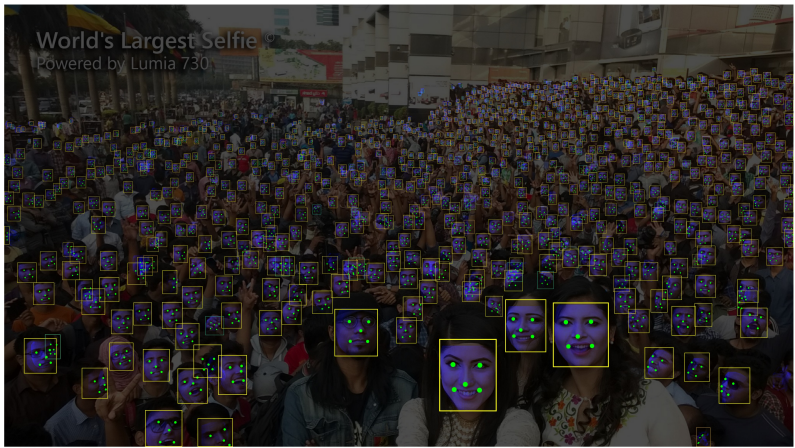
\includegraphics{obrazky-figures/RetinaFace.png}}
    \caption{Ukážka výstupu RetinaFace \cite{retinaface_ieee}.}
    \label{retina}
\end{figure}

Na obrázku \ref{retina} môžeme vidieť výstup z modelu RetinaFace. Jedná sa o selfie obrázok s najväčším počtom tvárí. RetinaFace dokázal nájsť okolo 900 ľudí z 1151. Maska žltej farby značí spoľahlivý výsledok, zatiaľ čo rámčeky tmavšej farby značia menej spoľahlivý výsledok \cite{retinaface_ieee}. 

\section{Rozpoznanie tváre}
V modernom svete sa čoraz viac spoliehame na technológie schopné identifikovať a rozpoznať objekty a osoby na základe vizuálnych dát. Rozpoznávacie algoritmy zohrávajú kľúčovú úlohu v mnohých aplikáciách, od bezpečnostných systémov a biometrických overení až po autonómne vozidlá a inteligentné zariadenia. Tieto algoritmy umožňujú systémom nielen vidieť, ale aj chápať a interpretovať vizuálny svet okolo nich \cite{facerec_3,facerec_2,facerec_1}.

V tejto sekcii sa pozrieme na niektoré rozpoznávacie algoritmy používané dnes. Patria sem ArcFace, DeepFace a FaceNet. Každý z týchto algoritmov prináša rôzne prístupy a techniky, ktoré umožňujú identifikáciu a overovanie tvárí. Preskúmame, ako tieto algoritmy fungujú, aké problémy riešia a v akých konkrétnych aplikáciách nachádzajú svoje uplatnenie.

\subsection{DeepFace}
DeepFace je model rozpoznávania tváre vyvinutí výskumníkmi z Facebooku. DeepFace bol trénovaný na označenom datasete o veľkosti viac ako 4 miliónov tvárí, čo bol najväčší súbor údajov o tvári v čase vydania. Prístup je založený na hlbokej neurónovej sieti s deviatimi vrstvami. Model dosahuje presnosť 97,35 \% na datasete LFW \cite{Deepface_rec_stranka}.

DeepFace ako stratovú funkciu využíva \textit{cross-enthropy}, namiesto aktivačnej funkcie \textit{sigmoid} využíva \textit{softmax}, v tvare \cite{Deepface_clanok}:
\begin{equation}
    L = -log(p_{k})
\end{equation}

\begin{equation}
    p_k = \frac{exp(o_k)}{\sum_h exp(o_h)}
\end{equation}

kde $p_k$ je výstup zo \textit{softmax} funkcie a $o_k$ je výstup poslednej plne pripojenej vrstvy \cite{Deepface_clanok}.

\subsection{FaceNet}
FaceNet je systém pre rozpoznávanie a verifikáciu tvárí. Dosahuje to učením mapovania z obrazov tvárí do euklidovského priestoru, kde sa na základe L2 vzdialenosti (podkapitola \ref{vektory}) určuje podobnosť tvárí. Táto vzdialenosť pre podobné snímky udáva nižšie hodnoty a pre rozdielne vyššie. FaceNet používa \textit{triplet loss}, čo umožňuje efektívne učenie sa rozdielov medzi tvárami. Táto stratová funkcia minimalizuje vzdialenosť medzi kotvou a pozitívnym príkladom (rovnaká identita) a maximalizuje vzdialenosť medzi kotvou (\textit{anchor}) a negatívnym príkladom (rôzna identita). \textit{Triplet loss} je definovaná ako \cite{facenet}:

\begin{equation}
    L = \sum_{i}^{N} \left[ \| f(x_a^i) - f(x_p^i) \|_2^2 - \| f(x_a^i) - f(x_n^i) \|_2^2 + \alpha \right]_+
    \label{eq:triplet_loss}
\end{equation}
kde:
\begin{itemize}
    \item $L$: Celková hodnota stratovej funkcie, ktorú minimalizujeme.
    \item $\sum_{i}^{N}$: Suma cez všetky vzorky v trénovacej množine.
    \item $N$: Počet vzoriek v trénovacej množine.
    \item $f(x)$: Funkcia, ktorá premieta obraz $x$ do vektorového priestoru.
    \item $x_a^i$: Ukotvený (\textit{anchor}) obraz vo vzorke $i$.
    \item $x_p^i$: Pozitívny obraz vo vzorke $i$ (obraz tej istej osoby ako ukotvený obraz).
    \item $x_n^i$: Negatívny obraz vo vzorke $i$ (obraz inej osoby než ukotvený obraz).
    \item $\| \cdot \|_2$: Euklidovská vzdialenosť (L2 vzdialenosť).
    \item $\alpha$: Okraj (\textit{margin}), ktorý oddeľuje pozitívne a negatívne páry.
    \item $[\cdot]_+$: Funkcia $\max(0, x)$, ktorá zaručuje, že príspevok k strate je nezáporný.
\end{itemize}

Na súbore dát LFW FaceNet dosiahol rekordnú presnosť 99,63 \%. Tento algoritmus sa široko používa v systémoch na overovanie identity a bezpečnostných aplikáciách, kde je potrebná rýchlosť a presnosť pričom \cite{facenet}.

\subsection{ArcFace}
ArcFace je algoritmus pre rozpoznávanie tvárí, ktorý optimalizuje presnosť pomocou \textit{Additive Angular Margin Loss}. Táto stratová funkcia je modifikáciou tradičnej \textit{softmax} stratovej funkcie. Oproti \textit{softmaxu} zahŕňa uhlovú penalizáciu, k výpočtu využíva funkciu arkus kosínus. Celkovo táto modifikácia umožňuje ArcFace lepšie zvládať prácu s nečistými dátami. Stratová funkcia ArcFace je definovaná ako \cite{arcface}:

\begin{equation}
    L = -\log \left( \frac{e^{s \cdot \cos(\theta_{y_i} + m)}}{e^{s \cdot \cos(\theta_{y_i} + m)} + \sum^N_{j \neq y_i} (e^{s \cdot \cos \theta_{j}}) } \right)
    \label{eq:rovnica_arcface}
\end{equation}

kde $\theta_{j}$ predstavuje úhol medzi váhou $W_j$ a vlastnosťou, $x_i$, $y_i$ je trieda i-tej vzorky, $s$ je škálovací faktor na kontrolu veľkosti vstupných vlastností a m je uhlová penalizácia. Na nasledujúcom obrázku \ref{arcloss} môžeme vidieť rozdiel stratových funkcií medzi \textit{Softmax} a ArcFace. Z obrázku \ref{arcloss} je vidieť lepšiu jednoznačnosť ArcFace oproti \textit{Softmax}. Práve vďaka tejto vlastnosti predstavuje ArcFace významnú úlohu pri rozpoznávaný tváre \cite{arcface}.

\begin{figure}[H]
    \centering
    \scalebox{0.55}{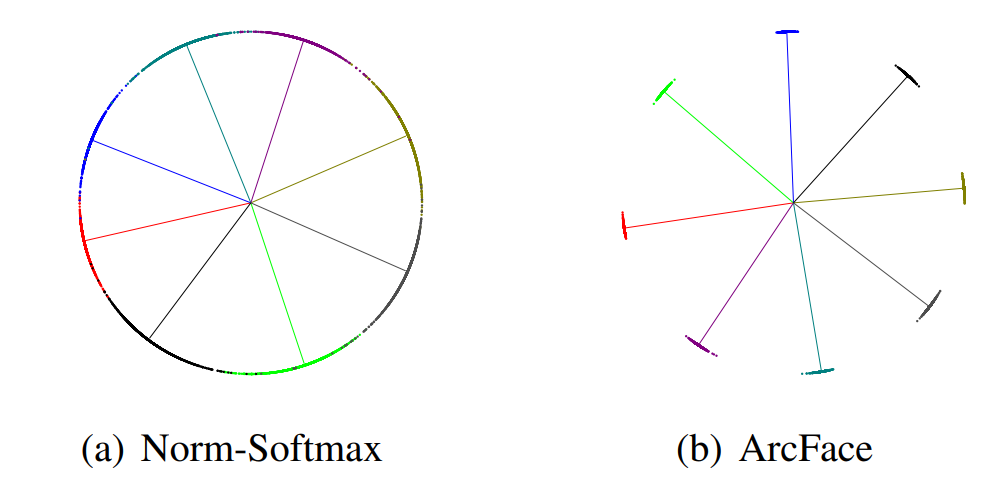
\includegraphics{obrazky-figures/arcloss.png}}
    \caption{Rozdiel stratovej funckie \textit{Softmax} a ArcFace \cite{arcface}.}
    \label{arcloss}
\end{figure}

Táto metóda zabezpečuje, že rozdiely medzi vektormi tvárí rôznych osôb sú maximalizované, čo zvyšuje spoľahlivosť rozpoznávania. ArcFace sa využíva v biometrických overovacích systémoch, kde je vysoká presnosť kľúčová, napríklad pri zabezpečení prístupu do citlivých oblastí \cite{arcface}.

\subsection{MagFace}
MagFace je algoritmus na rozpoznávanie tváre a pre hodnotenie kvality. Vychádza z ArcFace, kde sa snaží vytlačiť nejednoznačné vzorky preč z trénovacej množiny, aby sa zlepšil celkový výstup. K ArcFace stratovej funkcií pridáva uhlový okraj $m(a_i)$ a regularizátor $g(a_i)$. Uhlový okraj $m(a_i)$ sa stará o vyradzovanie menej kvalitných snímkov, pričom regularizátor $g(a_i)$ sa snaží docieliť, aby sa model hlavne učil na kvalitnejších snímkov. Stratová funkcia MagFace vyzerá nasledovne \cite{magface}:
\begin{equation}
    L = -\log \left( \frac{e^{s \cdot \cos(\theta_{y_i} + m(a_i)}}{e^{s \cdot \cos(\theta_{y_i} + m(a_i))} + \sum^N_{j \neq y_i} ( e^{s \cdot \cos \theta_{j}}) } \right) + \lambda_g g(a_i)
    \label{eq:magface_loss}
\end{equation}

kde $\theta_{j}$ predstavuje úhol medzi váhou $W_j$ a vlastnosťou, $x_i$, $y_i$ je trieda i-tej vzorky, $s$ je škálovací faktor na kontrolu veľkosti vstupných vlastností a m je uhlová penalizácia, táto časť je totožná s ArcFace. MagFace pridáva $m(a_i)$, čo predstavuje úhlový okraj, $g(a_i)$ regularizátor, ktorý oceňuje kvalitnejšie snímky a $\lambda_g$ je hyper-parameter pre balancovanie klasifikačnej a regulačnej straty \cite{magface}.

\subsection{Porovnanie embedding vektorov} \label{vektory}
Pri rozpoznávaní tváre sú \textit{embedding} vektory kľúčovým komponentom, ktorý umožňuje porovnávať rôzne tváre. Na porovnanie týchto vektorov sa používajú rôzne metriky vzdialenosti, medzi najčastejšie patrí Euklidovská $L2$ vzdialenosť, kosínusová vzdialenosť a Euklidovská $L2$ normovaná.

Euklidovská $L2$ vzdialenosť má nasledujúcu matematickú definíciu \cite{distance_embedding}:
\begin{equation}
    d(\overrightarrow{v}, \overrightarrow{w}) = \sqrt{\sum_{i}^{n} (v_i - w_i)^2}
    \label{eq:l2}
\end{equation}
kde $x$ a $y$ sú \textit{embedding} vektory dvoch tvárí. Používa sa na meranie priamej vzdialenosti medzi dvoma bodmi v n-rozmernom priestore. Čím je vzdialenosť vektorov menšia, tým je väčšia pravdepodobnosť, že sú si podobné \cite{distance_embedding}.

Kosínusová vzdialenosť má nasledujúcu matematickú definíciu \cite{distance_embedding}:
\begin{equation}
    cos(\beta) = \frac{\overrightarrow{v} \cdot \overrightarrow{w}}{\|\overrightarrow{v}\| \times \|\overrightarrow{w}\|}
    \label{eq:cos_dis}
\end{equation}
kde $v$ a $w$ sú \textit{embedding} vektory, $v \cdot w$ je skalárny súčin a $\|v\|$ je $L2$ norma vektora $v$. Používa sa na meranie uhla medzi dvomi vektormi, čím sa ohodnotí ich orientácia. Vhodná pre viac dimenzionálne priestory \cite{distance_embedding}.

Euklidovská $L2$ normovaná vzdialenosť má nasledujúcu matematickú definíciu \cite{wolfram}:
\begin{equation}
    \|\overrightarrow{v}\|_2 = \sqrt{\sum_{i}^{n} v_i^2}
    \label{eq:l2norm_dis}
\end{equation}
kde $v$ je \textit{embedding} vektor. Používa sa na normalizáciu vektorov, aby sa zabezpečilo, že všetky vektory majú rovnakú dĺžku. Normalizované vektory môžu byť následne porovnávané Euklidovskou alebo kosínusovou vzdialenosťou \cite{wolfram,l2norm}.

\subsection{Kľúčové metriky v oblasti rozpoznania tváre} \label{metrics}
V oblasti rozpoznania tváre, najmä pri detekcii deepfake, je nevýhnutné hodnotiť výkon rôznych algoritmov pomocou štandardných metrík pre binárnu klasifikáciu. Tieto metriky nám pomáhajú pochopiť ako dobre dokáže algoritmus vykonávať danú úlohu, v našom prípade ako dokáže rozlíšiť medzi skutočnými a zmanipulovanými deepfake obrazmi. Kľúčové metriky zahŕňajú \textit{True Positive}, \textit{True Negative} a presnosť \cite{TP_TN}.

\textit{True Positive} (TP) metrika predstavuje podiel prípadov, kedy algoritmus správne identifikuje pozitívny prípad. V našich experimentoch rozpoznania tváre ide o prípad, keď algoritmus správne identifikuje o dvoch skutočných obrázkov rovnakej osoby budú vyhodnotené, že patria tej istej osobe \cite{TP_TN}.

\textit{True Negative} (TN) metrika predstavuje podiel prípadov, kedy algoritmus správne identifikuje negatívny prípad. V našich experimentoch, práve vtedy keď ku skutočnému obrázku pôjde súčasne na vstup deepfake snímok, čiže výsledný výstup bude, že vstupné snímky neobsahujú rovnakú osobu \cite{TP_TN}. 

Výsledná presnosť, pre našu úlohu sa následne počíta ako:
\begin{equation}
    Accuracy = \frac{TP+TN}{Cases}
\end{equation}
kde \textit{Accuracy} je presnosť a \textit{Cases} značí počet prípadov. Vysoká presnosť naznačuje, že algoritmus je spoľahlivý v rozlišovaní medzi skutočnými obrázkami a deepfake\cite{TP_TN}.

\chapter{Návrh a implementácia}
Táto kapitola sa venuje návrhu a implementačnej časti tejto práce. V úvode práce bude popísaný návrh riešenia, ďalej sa pozrieme na nástroje a frameworky pre prácu s rozpoznaním tváre. Na záver je podrobnejší popis natrénovaných model konvolučných neurónových sietí.

\section{Návrh riešenia}
Nasledujúci obrázok \ref{diagram} obsahuje diagram aplikácie, ktorý si bližšie popíšeme. Na vstup aplikácie prichádzajú dva vstupné obrázky. Jeden z ktorého beriem tvár osoby (zdroj) a druhý referenčný na ktorý vložíme tvár zo zdroja. Z deepfake syntetizéru nám vypadne deepfake snímok. Ten spoločne s referenciou putuje do siamskej neurónovej siete a algoritmu rozpoznania tváre. V aplikácií je na výber z ArcFace, DeepFace, FaceNet a MagFace. Po tejto fáze dochádza k vyhodnoteniu výsledkov z oboch modelov.

\begin{figure}[H]
    \centering
    \scalebox{0.43}{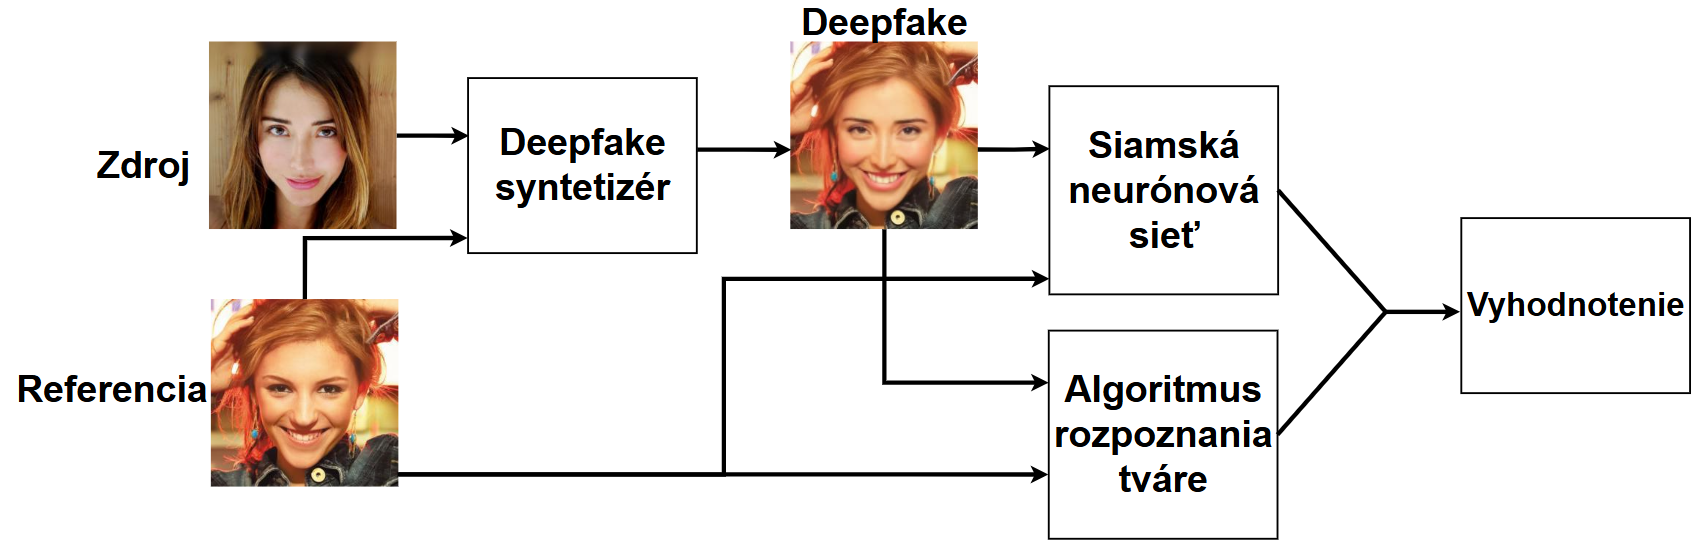
\includegraphics{obrazky-figures/Diagram_appky.png}}
    \caption{Diagram aplikácie.}
    \label{diagram}
\end{figure}

\section{Nástroje a frameworky}
Pre detekciu tváre existujú rôzne nástroje, ktoré obsahujú knižnice pracujúce s rozpoznaním tváre. Tieto nástroje nám môžu byť sprístupnené pomocou frameworku pre zjednodušenie práce s nimi. V tejto časti si popíšeme nástroje detekcie tváre a k nim 2 frameworky, využité pri implementácií tejto práce.

\subsection{Nástroje detekcie tváre a rozpoznávania}
Na detekciu tváre sa používajú rôzne nástroje. V nasledujúcom zozname si predstavíme zopár známych nástrojov detekcie \cite{face_rec_med2,face_detect}:
V tejto podsekcií si predstavíme zopár nástrojov používaných pre detekciu tváre.
\begin{itemize}
    \item Dlib\footnote{https://github.com/davisking/dlib}. Jedná sa o~\textit{toolkit} používaný v bezpečnosti a~analýze obrazu.
    \item Megvii Face++\footnote{https://en.megvii.com/technologies/face\_recognition} je často používaný pre kontrolu prístupu, elektronické obchodníctvo a~sociálne média.
    \item Deepface\footnote{https://github.com/serengil/deepface} je \textit{framework} pre Python, ktorý poskytuje analýzu tvárových vlastností ako je vek, pohlavie, rasa a~emocionálny stav.
    \item FaceNet\footnote{https://github.com/davidsandberg/facenet} vyvíjaný Googlom používa Python knižnice.
    \item InsightFace\footnote{https://github.com/deepinsight/insightface} je ďalšia Python knižnica dostupná na GitHube.
    \item OpenCV\footnote{https://opencv.org/} je \textit{open-source} Python knižnica pre počítačové videnie 
    \item PIL\footnote{https://pillow.readthedocs.io/en/stable/} je knižnica pre spracovanie obrázkov, implementovaná v jazyku Python.
\end{itemize}

\subsection{Knižnica TensorFlow a Keras API}
TensorFlow \cite{tensorflow2015-whitepaper} je \textit{open-source} knižnica pre strojové učenie vytvorená Googlom. TensorFlow sa používa na tvorenie a trénovanie modelov hlbokého učenia, pretože uľahčuje tvorbu výpočetných grafov a~zaisťuje efektívny beh modelov na rôznych druhoch hardwaru. Knižnica Tensorflow v sebe obsahuje populárne vysoko úrovňové aplikačné programové rozhranie (API) Keras \cite{chollet2015keras}. Keras poskytuje prístupné rozhranie pre riešenie problémov strojového učenia. Keras pokrýva každý krok postupu pri strojovom učení od spracovania cez ladenie až po nasadenie. Cieľ jeho vývoja bol umožniť rýchle experimentovanie pri tvorbe sietí.

\subsection{Frameworky}
Prvý framework, ktorý sme v rámci práci využili je Deepface. Umožňuje prepínať medzi niekoľkými \textit{state-of-art} modelmi ako sú FaceNet, ArcFace, a mnohé ďalšie. Tieto modely používa na detekciu, zarovnanie, reprezentáciu a overenie tváre. S pomocou pár riadkov kódu dokáže prispôsobiť rozpoznávanie tváre na úrovni ľudí \cite{deepface_teor}. Na nasledujúcom obrázku \ref{deepface_ukaz} môžeme vidieť ukážku výstupu Deepface frameworku.

\begin{figure}[H]
    \centering
    \scalebox{0.45}{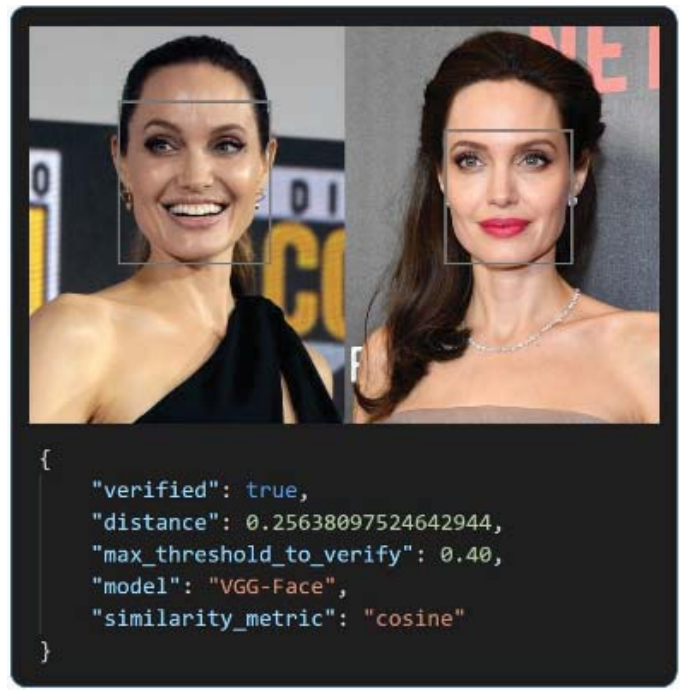
\includegraphics{obrazky-figures/deepface.png}}
    \caption{Výstup deepfacu pri overení tvári dvoch snímkov \cite{deepface_teor}.}
    \label{deepface_ukaz}
\end{figure}

Na obrázku môžeme vidieť výstup deepface, kde sa snaží zistiť, či tvár na dvoch snímkoch patrí rovnakej osobe. Na výstupe môžeme vidieť, že sa jedná o rovnakú osobu.

Druhý framework bola knižnica FaceAIKit \cite{face-ai-kit}, ktorá sa zameriava na detekciu a rozpoznanie tváre. Umožňuje jednoducho integrovať \textit{state-of-the-art} modely rozpoznania tváre. Pre detekciu tváre využíva RetinaFace a na rozpoznanie ArcFace alebo MagFace \cite{face-ai-kit}.

\section{Implementácia hodnotenia vierohodnosti}
Pre analýzu algoritmov rozpoznania tváre boli využité dva \textit{frameworky}, FaceAIKit a Deepface.

Prvý si popíšeme Deepface. Deepface ponúka na výber z troch funkcii na výpočet vzdialeností - kosínovskú, euklidovskú a L2 euklidovskú, pričom L2 by mala dosahovať najlepšie výsledky podľa autorov. Deepface obsahuje v sebe veľa modelov pre úlohy rozpoznania tváre, mi sme si vybrali FaceNet, DeepFace a ArcFace. Keď máme vybratý model a funkciu pre výpočet vzdialenosti môžeme zavolať funkciu \textit{verify}, ako môžeme vidieť v nasledujúcom úseku kódu \ref{deepface_verify}:

\begin{algorithm}[H]
\caption{Príklad práce s Deepface}
\begin{lstlisting}[language=Python]
result = DeepFace.verify(img1_path = reference, 
            img2_path = image, 
            model_name = "euclidean_l2",
            distance_metric = "Facenet")
\end{lstlisting}
\label{deepface_verify}
\end{algorithm}
V \textit{result} potom dostaneme výsledky vyhodnotenia, či sa referenčná osoba zhoduje s testovanou.

Druhý použitý \textit{framework} FaceAIKit pre výpočet vzdialenosti využíva tiež L2 euklidovskú vzdialenosť. FaceAIKit ponúka model ArcFace a MagFace. Knižnica sa na začiatku načíta a potom sú z nej volané funkcie ako môžeme vidieť na nasledujúcej ukážke \ref{deepface_verify_faceai}:
\begin{algorithm}[H]
\caption{Príklad práce s FaceAIKit}
\begin{lstlisting}[language=Python]
face_lib = FaceRecognition(recognition="arcface")

results1 = face_lib.face_detection(reference, align='keypoints')
results2 = face_lib.face_detection(image, align='keypoints')

distance = face_lib.verify(results1, results2)
\end{lstlisting}
\label{deepface_verify_faceai}
\end{algorithm}

Na základe hodnoty L2 sa potom určí či sa jedná o rovnaké osoby alebo nie.

\section{Návrh modelov}
Táto sekcia sa bude venovať návrhu modelu. Podrobnejšie si popíšeme architektúru siamskej siete, ktorá bola vychádzala z vedeckého článku. 

Návrh modelov s jedným vstupným snímkom obsahoval jednu sieť, ktorá bola poskytnutá skrz knižnicu TensorFlow ako môžeme vidieť v nasledujúcej ukážke \textit{Algorithm} \ref{vgg19_import}.

\begin{algorithm}[H]
\caption{Príklad so sieťou Vgg19}
\begin{lstlisting}[language=Python]
base_model = VGG19(include_top=False, input_shape=(128,128,3))
\end{lstlisting}
\label{vgg19_import}
\end{algorithm}

Schéma modelu potom vyzerá nasledovne \ref{vgg_navrh}:
\begin{figure}[H]
    \centering
    \scalebox{0.55}{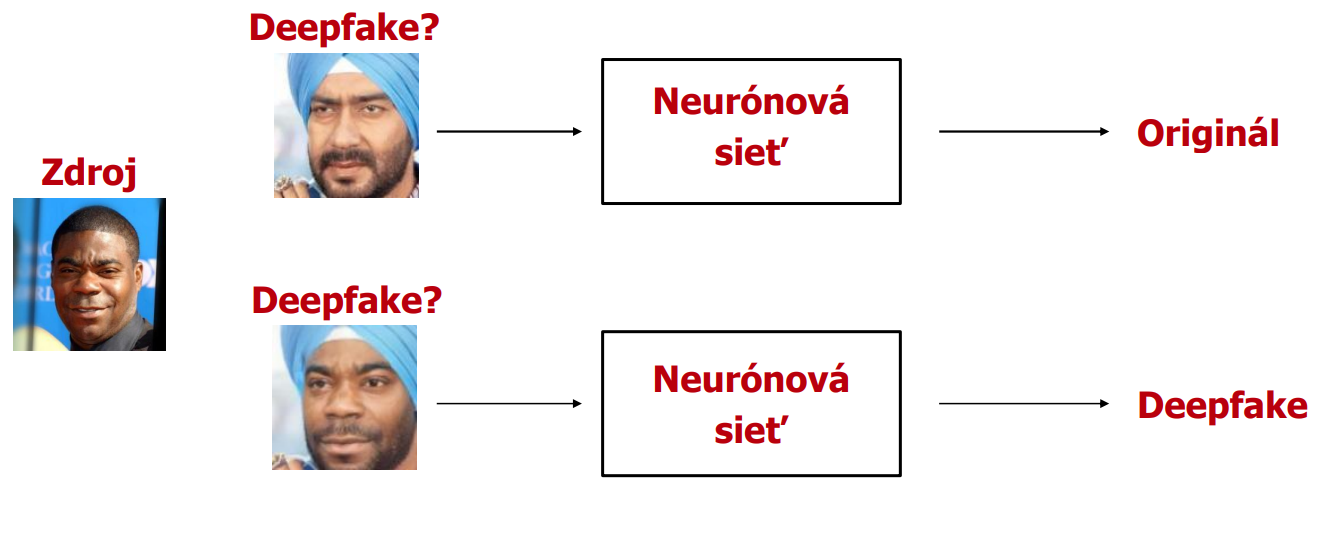
\includegraphics{obrazky-figures/Navrh_vgg.png}}
    \caption{Schéma návrhu modelu s jedným snímkom na vstupe.}
    \label{vgg_navrh}
\end{figure}

Na obrázku \ref{vgg_navrh} môžeme vidieť zdrojový obrázok, ktorý bol použitý pri vytvorení deepfaku. Prvý obrázok obsahuje originálny snímok a druhý je deepfake. Snímky idú do neurónovej siete, ktorá následne rozhodne či sa jedná o deepfake alebo nie.

Návrh siamskej siete bol komplexnejší a bol inšpirovaný článkom \cite{siam_obr}. Štruktúra súboru bola prevzatá z práce \cite{chollet2015keras}, z ktorej sme čerpali poznatky. Narozdiel od článkov sme nedefinovali vlastný model neurónovej siete, ale použili sme architektúru Vgg alebo ResNet. Predstavený model v článku \cite{chollet2015keras} nedosahoval dobré výsledky pre našu problematiku. Siete boli vložené do zdrojového kódu rovnako ako je naznačené v predchádzajúcej ukážke \textit{Algorithm} \ref{vgg19_import}. Podrobnejšie detaily implementácie sú popísané v nasledujúcej časti.

Schéma modelu siamskej siete vyzerá nasledovne \ref{siam_navrh}:
\begin{figure}[H]
    \centering
    \scalebox{0.50}{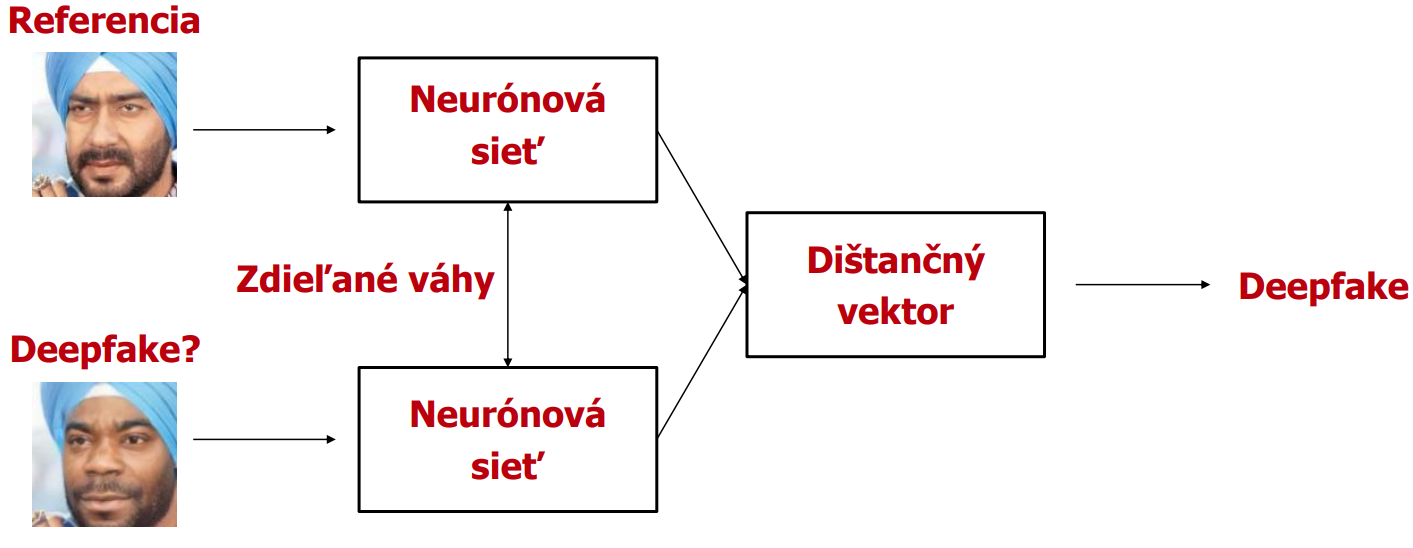
\includegraphics{obrazky-figures/Navrh_siamska.png}}
    \caption{Schéma návrhu modelu siamskej neurónovej siete.}
    \label{siam_navrh}
\end{figure}

Na obrázku \ref{siam_navrh} môžeme vidieť ako do modelu vstupujú dva vstupné snímky. Prvý z nich je vždy referencia a druhý je obrázok na porovnanie. Oba snímky idú do zvlášť neurónovej siete, avšak tieto dve siete zdieľajú váhy. Každá z nich pošle svoj výstup do dištančného vektora na základe jeho hodnoty sa určí výsledok.

\section{Implementácia a trénovanie modelu}
Výsledná aplikácia je tvorená v~programovacom jazyku Python, prevažne za použitia knižnice TensorFlow \cite{tensorflow2015-whitepaper} a Kerasu \cite{chollet2015keras}.

Po vytvorení datasetu sa začali vytvárať modely neurónových sietí. V rámci práce sú demonštrované pokusy na dvoch rôznych modelov neurónových sietí. Prvý model berie na vstup jeden vstupný snímok a~ako architektúru používa jednu sieť Vgg. Druhý model berie na vstup dva vstupné obrázky a~je vytvorený podľa schémy siamskej neurónovej siete z~vedeckého článku \cite{Koch2015SiameseNN}. 

Nami vytvorený dataset je uložený do dvoch priečinkov Deepfake a~Original. Deepfake priečinok obsahuje 4900 snímkov a~priečinok Original 1400 snímkov. V~položke Original sú snímky pomenované ako Origin\_{počet} a~v~položke deepfake ako Deep{X}\_{počet}, kde X značí o~ktorý deepfake algoritmus sa jedná, a~počet je poradové číslo snímky. Deep1 je pre program Roop, Deep2 pre program FaceFusion, Deep3 pre program Ghost a~Deep4 pre program SimSwap.

Trénovanie prvého modelu prebiehalo lokálne sa použitia grafickej karty RTX 3050 Ti. Verzia využitej TensorFlow knižnice bola 2.10.0 a~CUDA 11.2 pre grafickú akceleráciu. Model obsahuje funkciu z~knižnice TensorFlow, ktorá na základe pozície položky v~priečinku vygeneruje označenie pre dáta. Deepfake dáta sú označené číslom 0 a~originálne dáta sú označené číslom 1. Dáta sú potom normalizované, aby obsahovali hodnoty v~rozmedzí (0, 1), čo umožňuje rýchlejšiu konvergenciu modelu, pre lepšie trénovanie neurónovej siete. Následne sú dáta zamiešané a~rozdelené do trénovacích, validačných a~testovacích dát. Sú rozdelené v~pomere 70 \% pre trénovacie dáta, 20 \% pre validačné dáta a zvyšok je priradený testovacím dátam. Jednotlivé \textit{batche} obsahujú 32 snímkov, čo je východzia hodnota, ktorá bola pre našu problematiku dostačujúca. Ako architektúra neurónovej siete je použitá primárne, už spomínaná architektúra Vgg-net. V~experimentálnej časti sú popísané experimenty s~Vgg16 a~Vgg19. V rámci porovnania výsledkov boli využité aj siete ResNet, konkrétne ResNet50 a~ResNet101. Je možné naimportovať predtrénované váhy z~datasetu ImageNet do sietí alebo môžeme si váhy natrénovať samy na základe datasetu. Koncové vrstvy vynechávame, aby sme si ich mohli nadefinovať podľa seba. Ako poslednú vrstvu používame plne prepojenú vrstvu s funkciou sigmoid, ktorá sa hodí pre binárnu klasifikáciu. Optimalizátor je použitý Adam \cite{adam_opt} ako stratovú funkciu sme použili \textit{binary cross-entropy}, keďže klasifikujeme dva typy dát. 

Druhý model vyžadoval dataset uložiť ako páry dvoch obrázkov, keďže na vstup potrebujeme dva vstupné obrázky. Z~toho dôvodu sme sa rozhodli vytvoriť si vlastnú funkciu na načítanie dát a ich následné uloženie pre tréning siete. Dokopy je uložených 11200 párov z~nich 4900 je vytvorených spojením originálnych snímkov a~deepfake snímkov rovnakej osoby s~označením 1, ďalších 4900 je vytvorených spojením originálneho snímku s~deepfakom inej osoby s~označením 0 a~zvyšok je originál a~originál rovnakého človeka označení ako 0. Následne ako pri prvom modely sa jednotlivé snímky normalizujú na hodnotu v rozmedzí (0, 1) a~potom sa zamieša ich poradie. Rovnako ich pomer je 70 \% pre testovacie dáta, 20 \% pre validačné dáta a~zvyšok sú testovacie dáta. Veľkosť \textit{batchu} je nastavená na 64 snímkov. Architektúra modelu sa skladá z architektúry Vgg-net a~ResNet. Na vstup sa berie jeden pár snímkov, jednotlivý snímok z~páru ide cez Vgg sieť a~následne sa pomocou výsledku z~jednotlivej siete počíta dištančný vektor v~tvare $D = | dense1 - dense2 |$. Na nasledujúcom obrázku \ref{siam_navrh_podrob} môžeme vidieť podrobnejšie schéma na ktorom môžeme vidieť ako sa počíta spomínaný dištančný vektor.

\begin{figure}[H]
    \centering
    \scalebox{0.40}{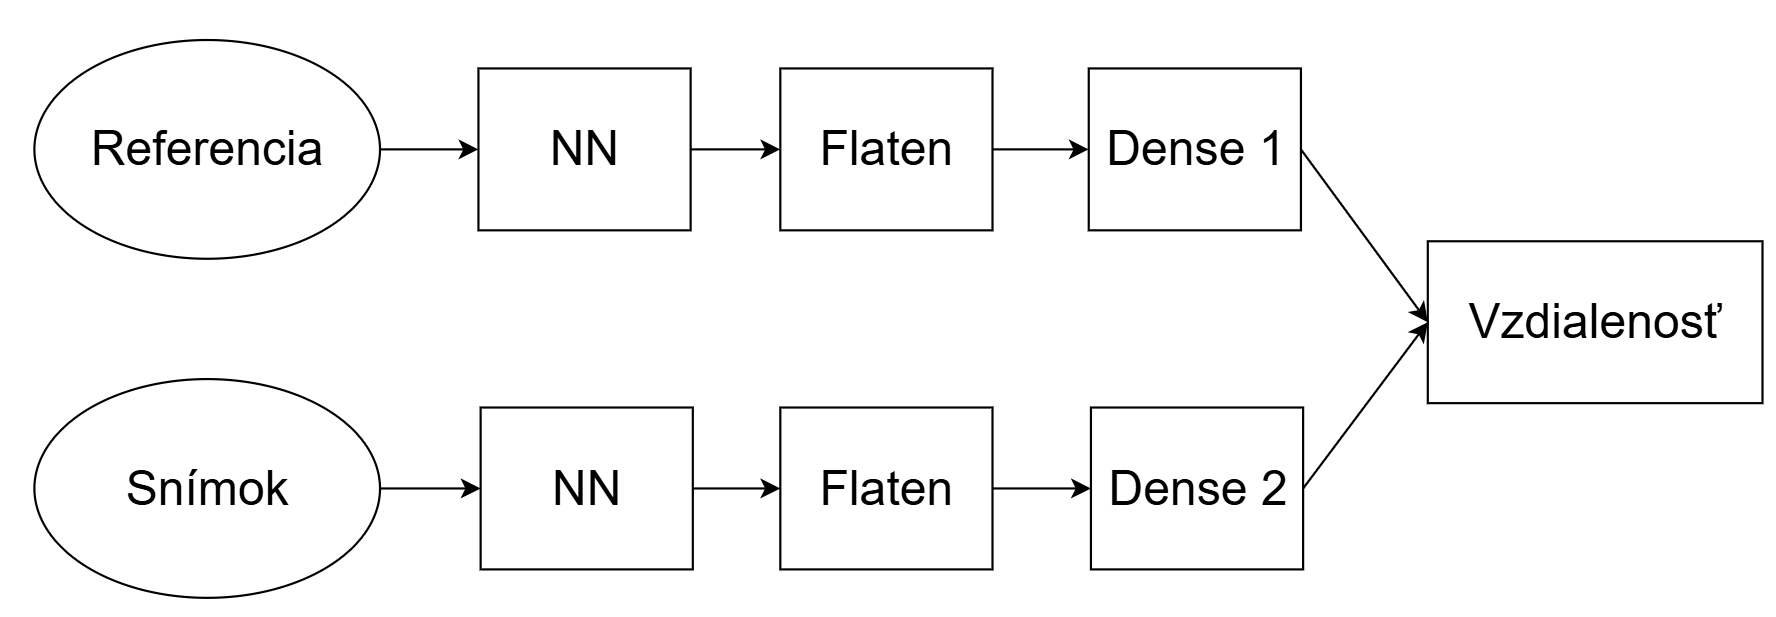
\includegraphics{obrazky-figures/Siamska_podrobnejsie.png}}
    \caption{Podrobnejšie schéma siamskej siete.}
    \label{siam_navrh_podrob}
\end{figure}

Na obrázku môžeme vidieť ako výstup jednotlivej siete ide do \textit{Flaten} vrstvy, ktorej výstup ide do \textit{Dense} na základe ich výstupu sa vypočíta dištančný vektor. Výsledný dištančný vektor ide do plne prepojenej vrstvy s~aktivačnou funkciou sigmoid. Optimalizér je použitý Adam, ktorý inicializujeme s rýchlosťou učenia $I_r = 1e-4$. Tento parameter ovplyvňuje veľkosť kroku počas optimalizácie, určujúc ako veľmi sú upravené parametri modelu v~každej iterácií tréningu. Ako stratové funkcie sme využili \textit{contrastive loss} a \textit{binary cross-entropy}.

\chapter{Experimenty a výsledky}
V~tejto kapitole sa venujeme experimentálnej časti práce. Na začiatku kapitoly bude popis prípravy datasetu, vytvárania deepfakov a zhrnutie použitých programov. Následne bude popis experimentov modelov neurónových sietí s rôznymi architektúrami a porovnanie ich výsledkov. Ďalej bude nasledovať vyhodnotenie experimentov algoritmov rozpoznania tváre a nakoniec vyhodnotenie dosiahnutých výsledkov.

\section{Príprava datasetu}
Dataset je dátový súbor, ktorý je organizovaný a~uložený spoločne pre analýzu alebo spracovanie. Datasety sú základným nástrojom v oblasti analýzy dát a~strojové učenie \cite{dataset}.

V~rámci implementácie bolo ako prvé treba vytvoriť vlastný deepfake dataset za použitia už existujúcich datasetov. Dáta pre náš dataset boli čerpané zo známeho datasetu ,ktorý sa často využíva pre prácu rozpoznania ľudí v~obraze, Labeled Faces in the Wild(LFW) \cite{LFWTech} a CelebA HQ \cite{liu2015faceattributes}. Dáta z týchto datasetov boli využité pre evaluáciu algoritmov. Z~LFW datasetu bolo vybraných 700 osôb ako cieľové obrázky pre tvorbu deepfake snímkov a~k~nim bolo náhodne vybraných 14 osôb, ktoré sa použili ako zdroj pre deepfake snímky. Tvár zdrojovej osoby je použitá na mapovanie 50 ľudí. Pri datasete CelebA bolo taktiež použitých 700 osôb aj s~rovnakým postupom tvorby deepfakov ako tomu bolo pri LFW. Dokopy boli použité 4 deepfake algoritmy pre väčšiu rozmanitosť deepfake datasetu a zaistenia väčšej robustnosti modelu neurónovej siete. Pre experimenty algoritmov rozpoznania tváre bol zvolený dataset CFP-FP.

\section{Tvorba deepfake}
V nasledujúcej sekcií si popíšeme jednotlivé použité deepfake algoritmy. Pri každom bude uvedený názov, pocity, vhodnosť a nakoniec zobrazíme ich výstupy.

\subsection{Deepfake program - Roop}
Prvý deepfake program, ktorý bol v tejto práci použitý sa nazýva Roop \cite{roop_algo}. Jedná sa o~\textit{open-source}, ktorý umožňuje vymieňať tváre ľudí na vstupe. Tento program poskytoval grafické užívateľské rozhranie (GUI), z ktorého bolo na prvý pohľad jasné ako sa má program používať. Pri výmene tvárí, keď boli značné rozdiely vo farbe alebo množstve vlasov na hlave, tak na výslednom obrázku vznikali viditeľné nedostatky vo vlasoch osôb, ktoré boli na prvý pohľad zjavne, že sa nejedná o~reálnu osobu, obrázok \ref{Deepfake_1_1}. Na obrázku \ref{Deepfake_1_2} môžeme vidieť výstup programu.

\begin{figure}[H]
    \centering
    \scalebox{0.43}{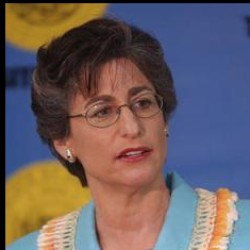
\includegraphics{obrazky-figures/Vzor1.jpg}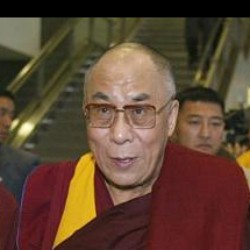
\includegraphics{obrazky-figures/Origin_206.jpg}
\includegraphics{obrazky-figures/Deep1_206.jpg}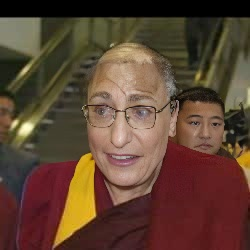
\includegraphics{obrazky-figures/Deep2_206.jpg}}
    \caption{Príklad problému s vlasmi -- Roop aj FaceFusion. Sprava prvý výsledok z FaceFusion, druhý sprava je z Roop.}
    \label{Deepfake_1_1}
\end{figure}

\begin{figure}[H]
    \centering
    \scalebox{0.45}{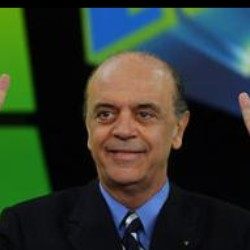
\includegraphics{obrazky-figures/Vzor2.jpg}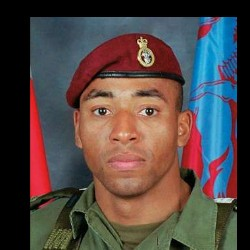
\includegraphics{obrazky-figures/Origin_57.jpg}
\includegraphics{obrazky-figures/Deep1_57.jpg}}
    \caption{Príklad výstupu -- Roop: zľava zdrojový obrázok, v strede je cieľový a vpravo je výsledný deepfake.}
    \label{Deepfake_1_2}
\end{figure}

\subsection{Deepfake program - FaceFusion} \label{face_fusion_rec}
Druhý deepfake program, ktorý bol v~tejto práci využití sa nazýva FaceFusion \cite{facefusion_algo}. Aplikácia obsahuje prehľadný návod na inštaláciu, čo ju umožňuje sprístupniť viacerým ľudom. Aplikáciu hodnotím pozitívne, pocitovo sa aj príjemnejšie ovládala a po skončení bolo ihneď vidieť výsledok v GUI aplikácie. Na obrázku \ref{Deepfake_2} môžeme vidieť výstup programu.


\begin{figure}[H]
    \centering
    \scalebox{0.45}  {
\includegraphics{obrazky-figures/Vzor3.jpg}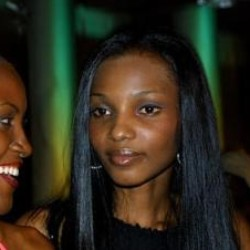
\includegraphics{obrazky-figures/Origin_41.jpg}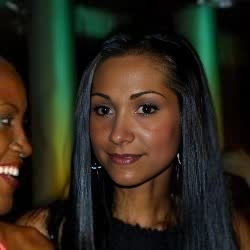
\includegraphics{obrazky-figures/Deep2_41.jpg}}
    \caption{Príklad výstupu -- FaceFusion: zľava zdrojový obrázok, v strede je cieľový a vpravo je výsledný deepfake.}
    \label{Deepfake_2}
\end{figure}

\newpage

\subsection{Deepfake program - Ghost}
Tretí použitý program pre tvorbu deepfake snímkov v~tejto práci bol Ghost \cite{ghost_deep}. Jednalo sa o konzolovú aplikáciu. Neobsahuje oproti predchádzajúcim aplikáciám GUI a~taktiež sa nedá nastaviť ktorú osobu, čo berieme za menšie negatívum. Proces tvorby deepfake snímkov bol vykonávaný rýchlejšie oproti predchádzajúcim aplikáciám. Program ako jediný zo všetkých použitých mal problémy vytvárať deepfake snímky za použitia datasetu CelebA HQ. V experimentálnej časti sme sa preto rozhodli využiť iba výstupy programu pre dataset LFW. Na obrázku \ref{Deepfake_3} môžeme vidieť výstup programu.

\begin{figure}[H]
    \centering
    \scalebox{0.5}  {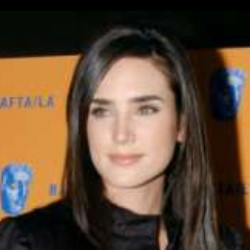
\includegraphics{obrazky-figures/Vzor4.jpg}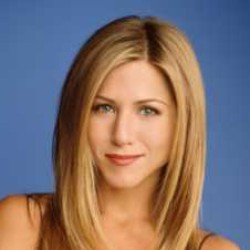
\includegraphics{obrazky-figures/Origin_601.jpg}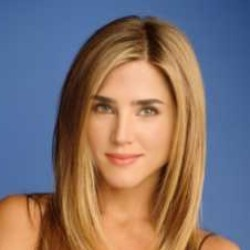
\includegraphics{obrazky-figures/Deep3_601.jpg}}
    \caption{Príklad výstupu -- Ghost: zľava zdrojový obrázok, v strede je cieľov a vpravo je výsledný deepfake.}
    \label{Deepfake_3}
\end{figure}

\subsection{Deepfake program - SimSwap}
Posledným použitým programom pre tvorbu deepfake snímkov bol SimSwap \cite{simswap_deep}. Jedná sa o~konzolovú aplikáciu tak ako tomu bolo pri Ghoste. Pri veľkej podobnosti osôb boli vytvorené výsledky dobrej kvality. Aplikáciu bolo náročné nainštalovať, jedná sa o~starší projekt, ktorý nie je extra udržiavaný. Celkový dojem radíme medzi horšie, najmä z dôvodu už spomínanej zaťaženej inštalácie programu. Na obrázku \ref{Deepfake_SimSwap} môžeme vidieť výstup programu.

\begin{figure}[H]
    \centering
    \scalebox{0.5}  {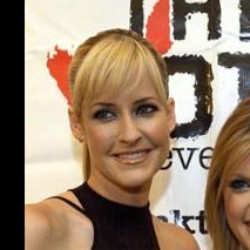
\includegraphics{obrazky-figures/Vzor7.jpg}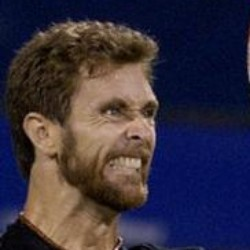
\includegraphics{obrazky-figures/Origin_327.jpg}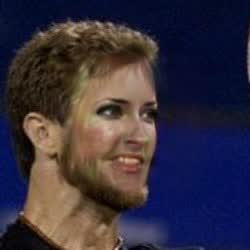
\includegraphics{obrazky-figures/Deep4_327.jpg}}
    \caption{Príklad výstupu -- SimSwap: zľava zdrojový obrázok, v strede je cieľov a vpravo je výsledný deepfake.}
    \label{Deepfake_SimSwap}
\end{figure}

Na nasledujúcom obrázku \ref{Deepfake_ukazky_vedla_seba} môžeme vidieť výstup všetkých deepfake programov, s cieľovými obrázkami aj s originálmi.

\begin{figure}[H]
    \centering
    \scalebox{0.43}{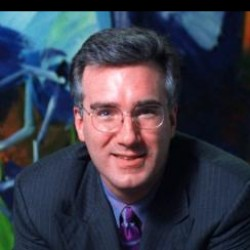
\includegraphics{obrazky-figures/Vzor5.jpg}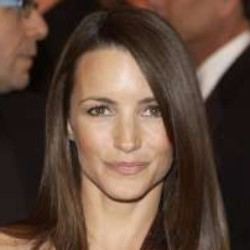
\includegraphics{obrazky-figures/Vzor6.jpg}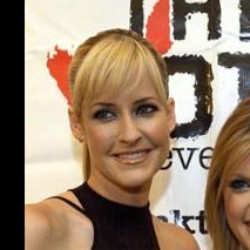
\includegraphics{obrazky-figures/Vzor7.jpg}}
    \scalebox{0.43}{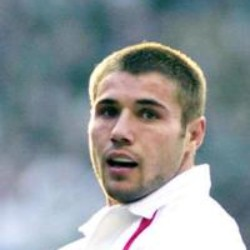
\includegraphics{obrazky-figures/Origin_144.jpg}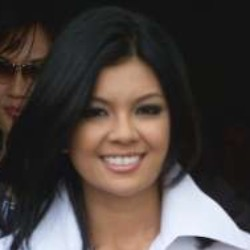
\includegraphics{obrazky-figures/Origin_171.jpg}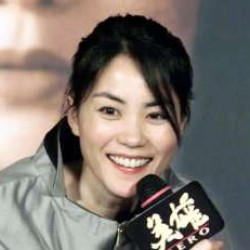
\includegraphics{obrazky-figures/Origin_315.jpg}}
    \scalebox{0.43}{
\includegraphics{obrazky-figures/Deep1_144.jpg}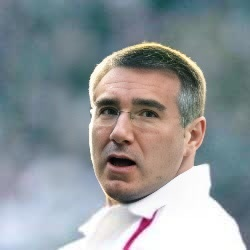
\includegraphics{obrazky-figures/Deep2_144.jpg}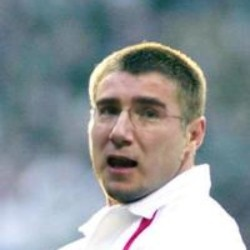
\includegraphics{obrazky-figures/Deep3_144.jpg}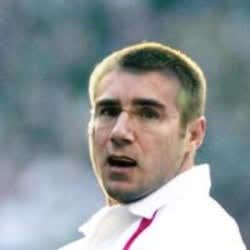
\includegraphics{obrazky-figures/Deep4_144.jpg}}
    \scalebox{0.43}{
\includegraphics{obrazky-figures/Deep1_171.jpg}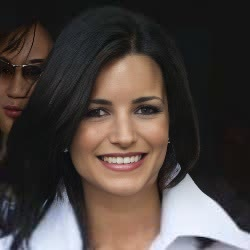
\includegraphics{obrazky-figures/Deep2_171.jpg}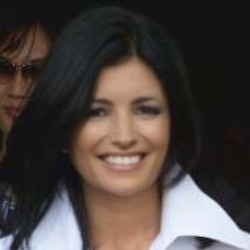
\includegraphics{obrazky-figures/Deep3_171.jpg}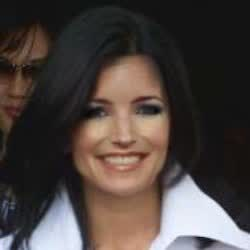
\includegraphics{obrazky-figures/Deep4_171.jpg}}
    \scalebox{0.43}{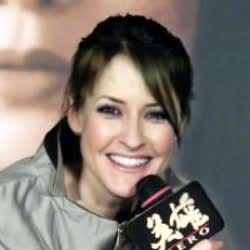
\includegraphics{obrazky-figures/Deep1_315.jpg}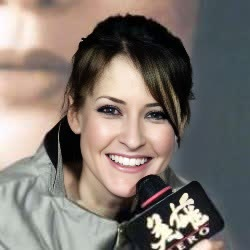
\includegraphics{obrazky-figures/Deep2_315.jpg}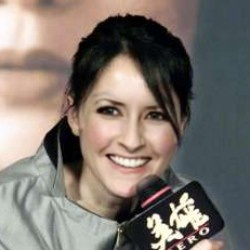
\includegraphics{obrazky-figures/Deep3_315.jpg}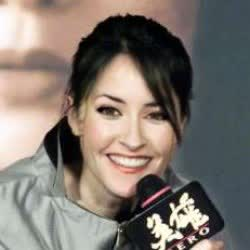
\includegraphics{obrazky-figures/Deep4_315.jpg}}
    \caption{Prvý riadok obsahuje snímky s tvárami osôb pre tvorbu deepfake. Druhý riadok obsahuje cieľové snímky. Pod prvým riadkom sú jednotlivé výstupy deepfakov -- Zľava originál, nasleduje roop, FaceFusion, Ghost, SimSwap. }
    \label{Deepfake_ukazky_vedla_seba}
\end{figure}

\section{Orezanie datasetu podľa tváre}
Po úspešnom vytvorení deepfake snímkov a~usporiadaným datasetu sa pred samotným implementovaní modelu neurónovej siete sme najskôr samotný LFW dataset zmenšili z pôvodnej veľkosti $250\times250$ na $128\times128$. Dataset CelebA obsahoval snímky veľkosti $256\times~256$, ktoré taktiež boli zmenšené na $128\times128$. To isté sme vykonali aj pre testovací dataset CFP-FP. Cieľ zmenšenia jednotlivých snímkov bolo, aby sa neurónová sieť zameriavala primárne na črty ľudskej tváre, aby sme dospeli k~lepším výsledkom. Orezávanie obrázka bolo vykonané za použitia \textit{open-sourc}e projektu autocrop \cite{autocrop} dostupného na GitHube. Algoritmus fungoval rovnako úspešne pre pôvodné obrázky ako aj pre deepfake snímky. Občas nejaké snímky orezal chybne alebo vôbec. Jednalo sa asi o~5 \% datasetu, tieto snímky boli napokon orezané ručne. Ukážka výsledných snímkov na obrázku \ref{Deepfake_ukazky_orezane_vedla_seba}.

\begin{figure}[H]
    \centering
    \scalebox{0.8}{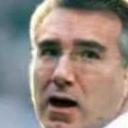
\includegraphics{obrazky-figures/crop_Deep1_144.jpg}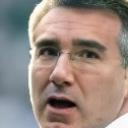
\includegraphics{obrazky-figures/crop_Deep2_144.jpg}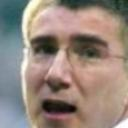
\includegraphics{obrazky-figures/crop_Deep3_144.jpg}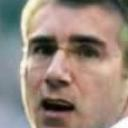
\includegraphics{obrazky-figures/crop_Deep4_144.jpg}}
    \scalebox{0.8}{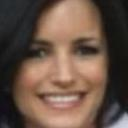
\includegraphics{obrazky-figures/crop_Deep1_171.jpg}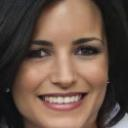
\includegraphics{obrazky-figures/crop_Deep2_171.jpg}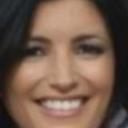
\includegraphics{obrazky-figures/crop_Deep3_171.jpg}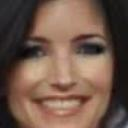
\includegraphics{obrazky-figures/crop_Deep4_171.jpg}}
    \scalebox{0.8}{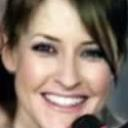
\includegraphics{obrazky-figures/crop_Deep1_315.jpg}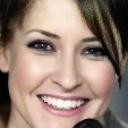
\includegraphics{obrazky-figures/crop_Deep2_315.jpg}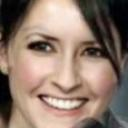
\includegraphics{obrazky-figures/crop_Deep3_315.jpg}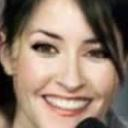
\includegraphics{obrazky-figures/crop_Deep4_315.jpg}}
    \caption{Ukážka finálneho stavu datasetu pred samotným trénovaním modelu neurónovej siete.}
    \label{Deepfake_ukazky_orezane_vedla_seba}
\end{figure}

\section{Model za použitia jednej siete architektúry Vgg-Net}\label{sec}
V~tejto sekcií si popíšeme výsledky konfigurácií použitia siete Vgg s~jedným vstupným snímkom. Tento model dostával postupne na vstup snímky po jednom a na ich základe sa snažil naučiť črty tváre, pre rozoznanie deepfake snímku od skutočného. Experimenty boli prevedené s obomi verziami siete Vgg a s dvomi verziami siete ResNet, konkrétne ResNet50 a ResNet101. Taktiež bolo vyskúšané použitie predtrénovaných váh ImageNet. 

Pred samotnou výslednou tabuľkou si popíšeme ako sme dostali výsledné hodnoty v tabuľkách \ref{tab:vgg_results} a \ref{tab:resnet_results}. Trénovanie modelov bolo nastavené na 50 epóch. Prvý stĺpec tabuľky obsahuje názov využitej architektúry neurónovej siete. Druhý stĺpec obsahuje hodnotu ImageNet alebo None. ImageNet udáva využitie predtrénovaných váh z datasetu ImageNet a None udáva, že neboli využité žiadne predtrénované váhy. Ďalšie stĺpce (Roop, Face, Ghost, Sim) obsahujú názov využitého deepfake programu pre tvorbu deepfake snímkov. Percentuálna úspešnosť udáva v koľkých percentách prípadoch správne klasifikoval vstupný snímok, táto hodnota bola vypočítaná ako aritmetický priemer predchádzajúcich stĺpcov tabuľky. Príklad ak na vstup prišiel deepfake a neurónová sieť určila, že sa o deepfake jedná percentuálna úspešnosť sa zvýšila. Ak výstup z nejakého z deepfake programov model určil ako originálny úspešnosť sa nezvýšila. Podobne je tomu aj pri stĺpci Origin, kde sa snažíme zistiť v koľkých prípadoch neurónová sieť správne určí, že vstupný snímok je originál a nie deepfake. Posledný stĺpec uvádza aritmetický priemer predchádzajúcich hodnôt, aby sme následne boli schopný modely medzi sebou porovnať. Na testovanie bolo využitých 500 snímkov. 100 originálnych snímkov a dokopy 400 deepfakov, pričom 100 snímkov bol výstup z každého deepfake programu. 50 snímok bolo z datasetu LFW a 50 z datasetu CelebA HQ. V nasledujúcej tabuľke \ref{tab:vgg_results} môžeme vidieť výsledok experimentov so sieťou Vgg:

\begin{table}[H]
\centering
\begin{tabular}{|l|c|c|c|c|c|c|c|}
\hline
\textbf{Model} & \textbf{Váhy} & \textbf{Roop} & \textbf{Face} & \textbf{Ghost} & \textbf{Sim} & \textbf{Origin} & \textbf{Suma}\\
\hline
Vgg16 & ImageNet & 100 \% & 87 \% & 91 \% & 88 \% & 38 \% & \textbf{80,8} \% \\
\hline
Vgg16 & None & 100 \% & 75 \% & 88 \% & 88 \% & 41 \% & 78,4 \% \\
\hline
Vgg19 & ImageNet & 100 \% & 75 \% & 88 \% & 88 \% & 41 \% & 78,4 \% \\
\hline
Vgg19 & None & 100 \% & 65 \% & 71 \% & 82 \% & 57 \% & 75,0 \% \\
\hline
\end{tabular}
\caption{Výsledky experimentov so sieťou Vgg.}
\label{tab:vgg_results}
\end{table}

Z výsledkov môžeme vidieť, že modely mali najväčší problém s klasifikáciou originálnych snímkov. Prvý deepfake algoritmu určili všetky konfigurácie bez problémov, pri ostatných sa výsledky líšili podľa zvolenej konfigurácie. Najúspešnejší model bol za použitia siete Vgg16 s využitím predtrénovaných váh ImageNet, ktorý dosiahol úspešnosť 80,8 \%. Na nasledujúcej tabuľke \ref{tab:resnet_results} môžeme vidieť výsledky experimentov so sieťou ResNet. Sieť ResNet sa pri tejto úlohe neosvedčila, nebola vôbec schopná správne určiť kedy sa jedná o originálny snímok. Mala tendenciu označovať všetky vstupné snímky ako deepfake.

\begin{table}[H]
\centering
\begin{tabular}{|l|c|c|c|c|c|c|c|}
\hline
\textbf{Model} & \textbf{Váhy} & \textbf{Roop} & \textbf{Face} & \textbf{Ghost} & \textbf{Sim} & \textbf{Origin} & \textbf{Suma}\\
\hline
ResNet50 & ImageNet & 100 \% & 92 \% & 99 \% & 96 \% & 0,1 \% & 77,5 \% \\
\hline
ResNet50 & None & 100 \% & 93 \% & 99 \% & 99 \% & 0,1 \% & 78,2 \% \\
\hline
ResNet101 & ImageNet & 100 \% & 97 \% & 100 \% & 99 \% & 0 \% & 79,2 \% \\
\hline
ResNet101 & None & 100 \% & 96 \% & 100 \% & 99 \% & 0,1 \% & 79,0 \% \\
\hline
\end{tabular}
\caption{Výsledky experimentov so sieťou ResNet.}
\label{tab:resnet_results}
\end{table}

Prvá sada experimentov ukázala, že aj za použitia iba jednej konvolučnej neurónovej siete je možné vytvoriť jednoduchý deepfake detektor. V~rámci experimentov sme vyskúšali rôzne konfigurácie sietí, kde najlepšie výsledky boli dosiahnuté pomocou siete Vgg16. ResNet architektúra sa pri tejto úlohe neosvedčila, čo môže byť spôsobené veľkou komplexnosťou siete pre našu úlohu. Celkovo konfigurácie dosahovali úspešnosť okolo 78 \%. V~nasledujúcej kapitole prevedieme rovnaké experimenty, ale budeme využívať architektúru siamskej siete.

\section{Model za použitia siamskej neurónovej siete}
V tejto časti si popíšeme experimenty s rôznymi architektúrami neurónových sietí s cieľom vybrať najlepší. Ten následne použijeme pri vyhodnotení výsledkov algoritmov rozpoznania tváre. Oproti predchádzajúcemu experimentu \ref{sec} siamské siete berú na vstup minimálne dva vstupné snímky, referenciu a potenciálny deepfake snímok. Trénovanie prebiehalo na externom výpočetnom stroji, ktorý bol poskytnutí Metacentrom\footnote{https://metavo.metacentrum.cz/}. Trénovanie bolo nastavené na 35 epoch všetkých experimentov, po trénovaný modely dosahovali vysoké presnosti. Veľkosť \textit{batchu} bola nastavená na 64. Do modelov vstupovali počas trénovania a validácie jednotlivé páry z celkového počtu 11200. 4900 párov obsahovalo deepfake a referenciu osoby, ktorá bola využitá pre tvorbu deepfake, 4900 párov boli referencia a deepfake inej osoby z nášho datasetu a~zvyšok snímkov obsahoval referenciu a rovnakú referenciu, čiže istý obrázok reálnej osoby.

V rámci experimentov boli skúšané dve rôzne stratové funkcie, a~to konkrétne \textit{binary cross-entropy} a \textit{contrastive loss}. \textit{Binary cross-entropy} bola použitá z knižnice TensorFlow a \textit{contrastive loss} sme si museli implementovať, na základe rovnice \ref{eq:rovnica4}.

Nasledujúce tabuľky budú obsahovať výsledky rôznych architektúr na trénovacích a validačných dátach. Do modelu vstúpia dva vstupné obrázky. Jeden referenčný, druhý potenciálny deepfake. Model má za úlohu správne klasifikovať druhý obrázok (potencionálny deepfake). Ak je pôvod obrázku Deepfake a model správne určí, že sa o deepfake jedná, tak sa zvyšuje percentuálna hodnota. Ak bol snímok deepfake a model ho určí ako originálny snímok hodnota sa nezvyšuje. Obdobne je tomu je pre originálne snímky, len naopak, kde sa snažíme určiť v koľkých percentách prípadov model správne určí, že sa jedná o originálny snímok. Schéma modelu je možné vidieť na obrázku \ref{siam_navrh}.

Prvý stĺpec tabuľky obsahuje názov architektúry neurónovej siete. Druhý stĺpec obsahuje váhu, teda či boli využité predtrénované váhy z datasetu ImageNet alebo nie. Tretí stĺpec obsahuje využitú stratovú funkciu, konkrétne buď \textit{binary cross-entropy} alebo \textit{contrastive loss}. Ďalšie stĺpce obsahujú výsledky vyhodnocovania pre jednotlivé deepfake programy -- Roop, Face, Ghost Sim. Predposledný stĺpec obsahuje výsledky pre originálne snímky. Posledný stĺpec obsahuje priemer predchádzajúcich hodnôt pre porovnanie celkovej úspešnosti modelov medzi sebou. Na základe tejto hodnoty sa vyberie najlepší model, ktorý bude ďalej využitý pri vyhodnocovaní experimentov. Dáta pre experimenty boli využité rovnaké ako v predchádzajúcej sekcií \ref{sec}. Nasledujúca tabuľka \ref{tab:siamese_vgg_results} obsahuje výsledky experimentov so sieťou Vgg.

\begin{table}[H]
\begin{tabular}{|l|c|c|c|c|c|c|c|c|}
\hline
\textbf{Model} & \textbf{Váhy} & \textbf{Strat} & \textbf{Roop} & \textbf{Face} & \textbf{Ghost} & \textbf{Sim} & \textbf{Origin} & \textbf{Suma}\\
\hline
Vgg16 & ImageNet & Cross & 82 \% & 62 \% & 60 \% & 44 \% & 72 \% & 64 \% \\
 &  & Contrast & 81 \% & 67 \% & 64 \% & 56 \% & 70 \% & 67,6 \%\\
 \hline
Vgg16 & None & Cross & 87\% & 68 \% & 66 \% & 57 \% & 67 \% & \textbf{69} \% \\
 &  & Contrast & 85 \% & 67 \% & 64 \% & 53 \% & 69 \% & 67,6 \%\\
\hline
Vgg19 & ImageNet & Cross & 77 \% & 65 \% & 52 \% & 67 \% & 71 \% & 66,4 \% \\
 &  & Contrast & 62 \% & 48 \% & 34 \% & 49 \% & 87 \% & 56 \%\\
 \hline
Vgg19 & None & Cross & 80 \% & 67 \% & 52 \% & 68 \% & 70 \% & 67,4 \% \\
 &  & Contrast & 75 \% & 61 \% & 54 \% & 68 \% & 73 \% & 66,2 \%\\
\hline
\end{tabular}
\centering
\caption{Výsledky experimentov siamskej siete so sieťou Vgg.}
\label{tab:siamese_vgg_results}
\end{table}

Celkové výsledky zaznamenali horšie hodnoty oproti predchádzajúcemu experimentu. Jednotlivé stratové funkcie udávali podobné úspešnosti. Pri určovaný originálnych snímkov sa výstup zlepšil o mnoho oproti predchádzajúcim experimentom. Siamská sieť mala väčší problém správne určovať deepfake snímky. Najlepší model dokázal správne klasifikovať 69 \% testovacieho datasetu. Využíval sieť Vgg16 bez predtrénovaných váh so stratovou funkciou \textit{binary cross-entropy}. Pri experimentoch siamskej siete sme sa rozhodli nevyužiť sieť ResNet. Model sa natrénoval, ale nedosahoval dobré úspešnosti obdobne ako v predchádzajúcich experimentoch. Taktiež potreboval väčší výpočetný výkon čo spôsobilo, že sa nedal zakomponovať do výslednej aplikácie. V nasledujúcej časti vezmeme z každej sekcie najlepší model a~vykonáme porovnanie s voľne dostupným deepfake detektorom BioID.  

\section{Porovnanie výsledkov s deepfake detektorom BioID}
V~tejto sekcií, vykonáme porovnanie nášho najlepšieho modelu za použitia jednej siete Vgg16. Cieľom experimentu je porovnať úspešnosť nášho modelu s komerčným deepfake detektorom od firmy BioID\footnote{https://www.bioid.com/}, ktorý je verejne dostupný.

Pre porovnanie výsledkov bolo náhodne vybraných 20 snímkov z testovacieho datasetu. Boli skúšané všetky kategórie snímkov - Originálne, Roop, Facefusion, Ghost a SimSwap. V~nasledujúcej tabuľke \ref{tab:BioID_table} môžeme vidieť jednotlivé percentuálne úspešnosti správnej klasifikácie testovacieho datasetu.

\begin{table}[htbp]
\begin{tabular}{|l|c|c|c|c|c|c|}
\hline
\textbf{Model} & \textbf{Roop} & \textbf{FaceFusion} & \textbf{Ghost}  & \textbf{SimSwap} &  \textbf{Originál} & \textbf{Celkovo}\\
\hline
BioID & 20 \% & 50 \% & 65 \% & 40 \% & 60 \% & 47 \% \\
\hline
Vgg16 & 85 \% & 90 \% & 90 \% & 85 \% & 40 \% & 78 \% \\
\hline
\end{tabular}
\centering
\caption{Výsledky porovnania nášho modelu s BioID.}
\label{tab:BioID_table}
\end{table}

Do BioID detektoru bolo nutné posielať na vstup neorezané snímky, pri orezaných bola vyhodená chyba. Detektor od BioID primal na vstup jeden snímok na základe ktorého sa rozhodoval, či sa jedná o deepfake alebo nie, podobne ako náš Vgg16 model. Najťažšia úloha pre BioID detektor bola rozoznať snímky vygenerované deepfake programami SimSwap a Roop. Túto skutočnosť môžeme vidieť vo výslednej tabuľke \ref{tab:BioID_table}. V~rámci porovnania skončil deepfake detektor od BioID horšie ako náš natrénovaný model. Je zvláštne, že BioID mal tendenciu klasifikovať väčšinu snímkov, vytvorených pomocou programu SimSwap a~Roop za originál a~originálne pomerne často naopak za deepfake. Na výsledkoch môžeme vidieť, že sa nejedná o jednoduchú úlohu správne rozlíšiť deepfake od originálnych snímkov.

\section{Experimenty algoritmov pre rozpoznanie tváre}
V tejto časti budú popísané výsledky experimentov s algoritmami pre rozpoznanie tváre voči deepfakom. V rámci týchto experimentov sme si vytvorili dataset ktorý obsahoval dva snímky rovnakej osoby a jeden deepfake snímok ako môžeme názorne vidieť na nasledujúcom obrázku \ref{CFP_ukaz}:

\begin{figure}[H]
    \centering
    \scalebox{0.6}  {
\includegraphics{obrazky-figures/CFP_1.jpg}
\includegraphics{obrazky-figures/CFP_2.jpg}
\includegraphics{obrazky-figures/Deep_2.jpg}}
    \caption{Ukážka datasetu pre experimenty s algoritmami pre rozpoznanie tváre. Zľava referencia (\textit{Real1}), druhý snímok rovnakej osoby ako je na referencií (\textit{Real2}), deepfake predchádzajúceho snímku (\textit{Fake})}
    \label{CFP_ukaz}
\end{figure}

Pri tvorbe testovacieho datasetu sme vybrali dvojicu fotiek pre každú osobu z datasetu CFP-FP. Dokopy sme mali snímky 200 osôb, ku ktorým sme vytvorili jeden deepfake snímok, tak ako je zobrazené na ukážke na obrázku \ref{CFP_ukaz}. Pre tvorbu deepfake bol využitý program FaceFusion, podkapitola \ref{face_fusion_rec}. Následne sme pri algoritmov pre rozpoznanie tváre určovali presnosť, či je na oboch snímkoch rovnaká osoba. Ak na vstup prišli obrázky \textit{Real1} (1. obrázok v \ref{CFP_ukaz}) a \textit{Real2} (2. obrázok v \ref{CFP_ukaz}) výstup mal byť, že sa jedná o rovnakú osobu, a teda sa presnosť zvýšila. Ak výstup bol, že na obrázkoch nie sú rovnaké osoby presnosť zostala nezmenená. Podobne tomu bolo keď na vstup prišiel deepfake. Pri deepfake sme robili dva experimenty, kde na vstup išla \textit{Real1} a \textit{Fake} (3. obrázok v \ref{CFP_ukaz}) alebo \textit{Real2} a \textit{Fake}. Princíp bol rovnaký, keď algoritmus určil, že sa nejedná o rovnakú osobu presnosť sa zvýšila, ak tomu bolo naopak tak zostala nezmenená. Pri experimentoch sme skúšali dve rôzne techniky výpočtu dištančného vektora a to kosínusovú a Euklidovskú L2. Prvá tabuľka \ref{tab:Face_rec_table_l2} obsahuje výsledky Euklidovskej L2 vzdialenosti a druhá tabuľka \ref{tab:Face_rec_table_cos} obsahuje výsledky kosínovskej vzdialenosti. V zvlášť tabuľke \ref{tab:Face_rec_table_siamese} sme vykonali rovnaký experiment s naším najlepším modelom siamskej siete, aby sme porovnali výsledky s algoritmami pre rozpoznanie tváre. Bližší popis k metrikám v podkapitole \ref{metrics}. V tabuľke sú taktiež uvedené prahové hodnoty pre jednotlivé algoritmy pre rozpoznanie tváre, na základe ktorých sa určilo či sa jedná o rovnakú osobu alebo nie. Prahové hodnoty sú určené pre najlepšiu presnosť jednotlivých algoritmov.

\begin{table}[H]
\centering
\begin{tabular}{|l|c|c|c|c|}
\hline
\multirow{2}{*}{\textbf{Model a prah}} & \multicolumn{1}{|c|}{\textbf{True Positive}} & \multicolumn{2}{|c|}{\textbf{True Negative}} & \multirow{2}{*}{\textbf{Presnosť}} \\
\cline{2-4}
& \textbf{Real1 a Real2} & \textbf{Real1 a Fake} & \textbf{Real2 a Fake} & \\
\hline
FaceNet -- 0,8 & 74,5 \% & 100 \% & 100 \% & 91,5 \% \\
\hline
DeepFace -- 0,64 & 64 \% & 58,5 \% & 24,5 \% & 49 \% \\
\hline
ArcFace -- 1,13 & 95,5 \% & 99 \% & 94 \% & 96,2 \% \\
\hline
MagFace -- 1,1 & 100 \% & 100 \% & 100 \% & 100 \% \\
\hline
\end{tabular}
\caption{Výsledky experimentov algoritmov pre rozpoznanie tváre za použitia Euklidovskej L2 vzdialenosti.}
\label{tab:Face_rec_table_l2}
\end{table}

\begin{table}[H]
\centering
\begin{tabular}{|l|c|c|c|c|}
\hline
\multirow{2}{*}{\textbf{Model a prah}} & \multicolumn{1}{|c|}{\textbf{True Positive}} & \multicolumn{2}{|c|}{\textbf{True Negative}} & \multirow{2}{*}{\textbf{Presnosť}} \\
\cline{2-4}
& \textbf{Real1 a Real2} & \textbf{Real1 a Fake} & \textbf{Real2 a Fake} & \\
\hline
FaceNet -- 0,4 & 88,5 \% & 99,5 \% & 98,5 \% & 95,5 \% \\
\hline
DeepFace -- 0,23 & 72,5 \% & 46 \% & 18,5 \% & 45,6 \% \\
\hline
ArcFace -- 0,68 & 96,5 \% & 94 \% & 88 \% & 92,8 \% \\
\hline
\end{tabular}
\centering
\caption{Výsledky experimentov algoritmov pre rozpoznanie tváre za použitia Cos vzdialenosti.}
\label{tab:Face_rec_table_cos}
\end{table}

\begin{table}[H]
\centering
\begin{tabular}{|l|c|c|c|c|}
\hline
\multirow{2}{*}{\textbf{Model}} & \multicolumn{1}{|c|}{\textbf{True Positive}} & \multicolumn{2}{|c|}{\textbf{True Negative}} & \multirow{2}{*}{\textbf{Presnosť}} \\
\cline{2-4}
& \textbf{Real1 a Real2} & \textbf{Real1 a Fake} & \textbf{Real2 a Fake} & \\
\hline
Siamese & 89 \% & 56,5 \% & 91,5 \% & 79 \% \\
\hline
\end{tabular}
\centering
\caption{Výsledky experimentov siamskej siete pre porovnanie výsledkov voči algoritmom pre rozpoznanie tváre.}
\label{tab:Face_rec_table_siamese}
\end{table}

Z výsledkov môžeme vidieť, že väčšina algoritmov dosahovala dobré výsledky. Najhoršie skončil DeepFace a potom náš model siamskej siete. Náš model nepoužíval rôzne metriky na vyhodnocovanie experimentov, preto je uvedený zvlášť. Najlepší výsledok dosiahol MagFace s presnosťou 100 \%. Euklidovská vzdialenosť dosahovala všeobecne lepšie výsledky oproti kosínovskej, jedinou výnimkou bol FaceNet. MagFace má experimenty iba pomocou Euklidovskej vzdialenosti, lebo v použitej knižnici kosínus nebol dostupný. Jednotlivé algoritmy rozpoznania tváre sme vyniesli na grafy hustoty pravdepodobnosti pre Euklidovskú L2 vzdialenosť. Môžeme vidieť na nasledujúcich obrázkov grafov. Pre prehľadnosť násludujúce grafy budú pre Euklidovskú L2 vzdialenosť. Kosínus dosahoval podobné výsledky, ako môžeme vidieť v predchádzajúcich tabuľkách.

\begin{figure}[H]
    \centering
    \scalebox{0.53}{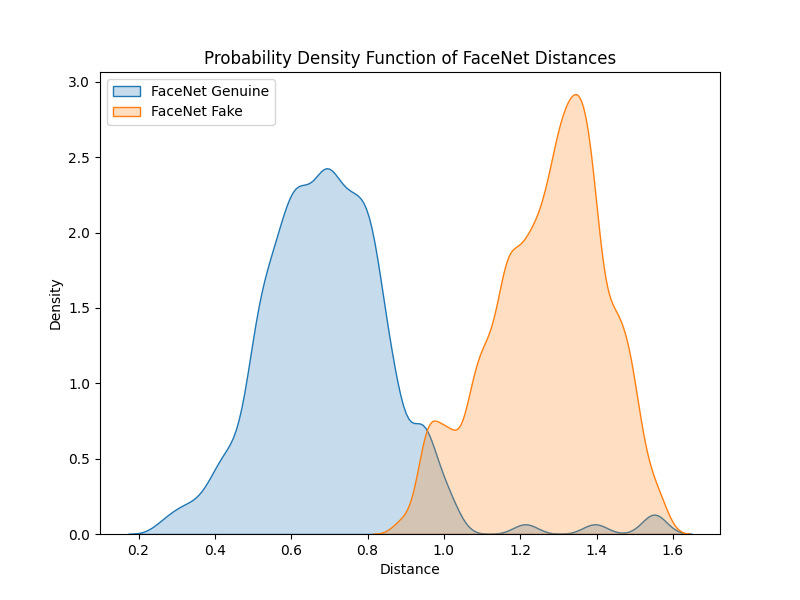
\includegraphics{obrazky-figures/FaceNet_L2_spolu.png}}
    \caption{Funkcia hustoty pravdepodobnosti v jednom grafe za použitia L2 vzdialenosti - FaceNet.}
    \label{FaceNet_L2_spolu}
\end{figure}

Na obrázku \ref{FaceNet_L2_spolu} môžeme vidieť rozdielne stredové hodnoty pre jednotlivé hodnoty. Modrá krivka znázorňuje hodnoty pre originálne snímky a oranžová pre deepfake. Väčšina snímkov bola zvlášť klasifikovaná, ale môžeme vidieť prekryv medzi hodnotami 0,8 až 1,0, kde snímky boli určované aj ako originálne, ale aj ako deepfake. Niektoré originálne snímky boli určené s veľkou vzdialenosťou, ktorá bola typickejšia pre deepfake snímky ako môžeme vidieť malé vlnky v modrom grafe. Prahová hodnota pre rozlíšenie, či sa jedná o rovnaké alebo rôzne osoby má FaceNet nastavenú na 0,8 pre Euklidovskú L2 vzdialenosť (obrázok \ref{FaceNet_L2_spolu}) a pre kosínovskú 0,4.

Na nasledujúcom grafe \ref{MagFace_L2_spolu} si ukážeme výstup MagFace, ktorý dosiahol najlepší výsledok v experimentoch:

\begin{figure}[H]
    \centering
    \scalebox{0.53}{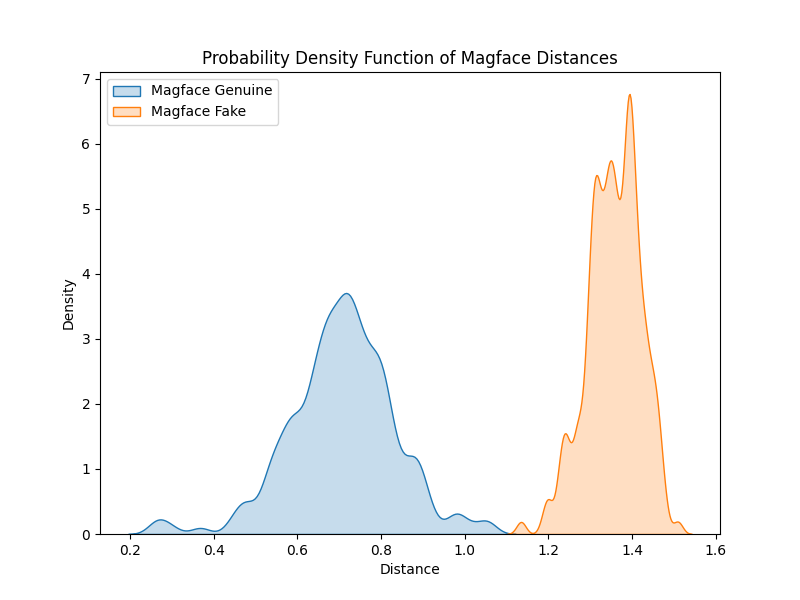
\includegraphics{obrazky-figures/MagFace_L2_spolu.png}}
    \caption{Funkcia hustoty pravdepodobnosti v jednom grafe za použitia L2 vzdialenosti - MagFace.}
    \label{MagFace_L2_spolu}
\end{figure}

Na grafe \ref{MagFace_L2_spolu} môžeme vidieť, že výstupy pre originály nemajú prienik hodnôt s výstupmi pre deepfake. Prahová hodnota pre MagFace je 1,1 pre Euklidovskú L2 vzdialenosť. Na nasledujúcom grafe \ref{DeepFace_L2_spolu} si môžeme výstupy porovnať s najhorším výsledok v rámci experimentov, ktorý bol dosiahnutý algoritmom DeepFace.

\begin{figure}[H]
    \centering
    \scalebox{0.53}{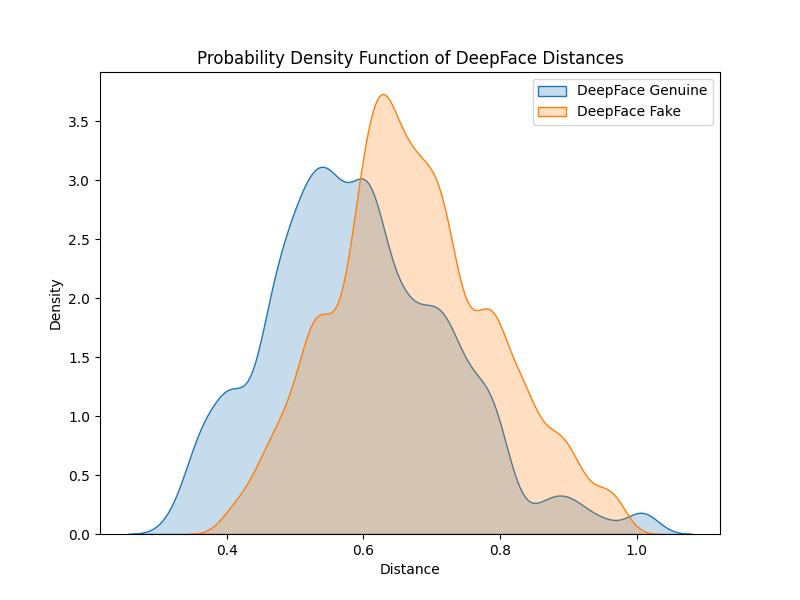
\includegraphics{obrazky-figures/DeepFace_L2_spolu.png}}
    \caption{Funkcia hustoty pravdepodobnosti v jednom grafe za použitia L2 vzdialenosti - DeepFace.}
    \label{DeepFace_L2_spolu}
\end{figure}

Na grafe \ref{DeepFace_L2_spolu} môžeme vidieť veľký prienik hodnôt. DeepFace má prahovú hodnotu nastavenú na 0,64 pri Euklidovskej L2 vzdialenosti a 0,23 pri kosínusovej. DeepFace nevedel spoľahlivo určiť, či sa na vstupných snímkoch nachádza rovnaká osoba. Tento fakt je viditeľný na grafe, keďže sa tam nachádza vysoký prienik hodnôt. DeepFace je najstarší z hodnotených algoritmov a od jeho vzniku pribudli mnohé ďalšie algoritmy pre rozpoznanie tváre, ktoré ho prekonávajú v rôznych \textit{benchmarkoch}. Na základe výsledkov sa jeho použitie neosvedčilo. Na poslednom obrázku \ref{ArcFace_L2_spolu} môžeme vidieť graf posledného testovacieho algoritmu ArcFace:

\begin{figure}[H]
    \centering
    \scalebox{0.53}{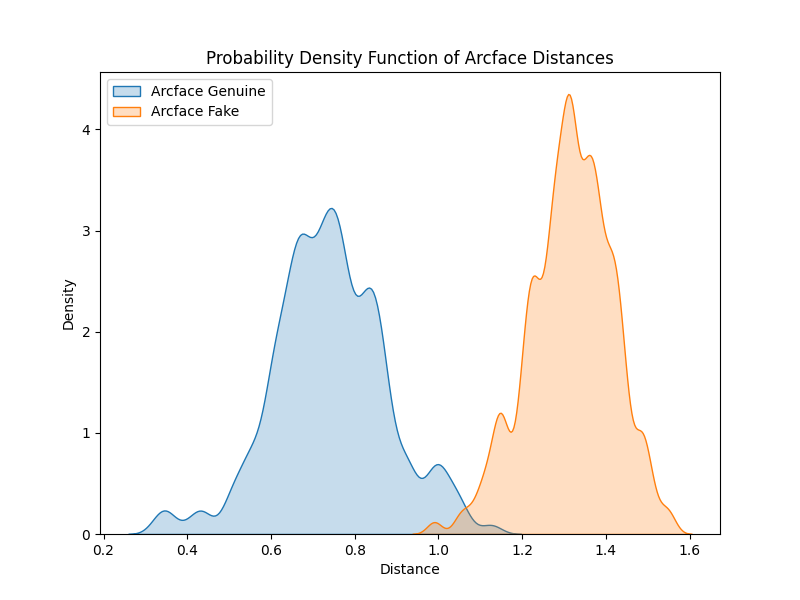
\includegraphics{obrazky-figures/ArcFace_L2_spolu.png}}
    \caption{Funkcia hustoty pravdepodobnosti v jednom grafe za použitia L2 vzdialenosti - ArcFace.}
    \label{ArcFace_L2_spolu}
\end{figure}

Na poslednom obrázku \ref{ArcFace_L2_spolu} môžeme vidieť graf ArcFace. ArcFace má prahovú hodnotu nastavenú na 1,13 pri Euklidovskej L2 vzdialenosti a 0,68 pri kosínusovej. ArcFace dosiahol druhý najlepší výsledok. Na grafe môžeme vidieť, že prienik hodnôt nebol vysoký.

Z experimentov vyplýva odolnosť určitých algoritmov pre rozpoznanie tváre voči deepfake. Najlepšie výsledky boli za použitia MagFace, kde presnosť dosahovala $100 \%$. Najhoršie výsledky boli za použitia DeepFace, kde model väčšinu snímkov vyhodnocoval na základe vzdialenosti ako deepfake. Náš model siamskej neurónovej siete bol schopný určovať či sa jedná o deepfake alebo nie, avšak výsledky boli slabšie oproti algoritmom rozpoznania tváre. Pri originálnych snímkoch na vstupe dával pomerne správne výsledky vo viac ako $91 \%$ prípadov. Podobný trend bol aj keď na vstup išla referencia a deepfake referencie. Akonáhle sme na vstup poslali inú referenciu ako bol deepfake snímok vytvorený, tak presnosť rapidne klesla. Poradie od najlepšieho modelu po najhorší na základe výsledkov je následovné: MagFace, ArcFace, FaceNet, Siamská sieť, DeepFace.

\newpage

\section{Zhrnutie výsledkov}
V~experimentálnej časti sme demonštrovali a~porovnali jednotlivé konfigurácie vytvorených modelov. Jednotlivé modely boli schopné klasifikovať, či sa jedná o~deepfake alebo nie, s rôznymi úspešnosťami. Z jednotlivých experimentov lepšie výsledky dosahovala sieť Vgg16 oproti Vgg19. Model, ktorý bral na vstup jeden vstupný snímok dosahoval úspešnosť okolo $80 \%$. Pri siamskej sieti úspešnosť klesla pod $70 \%$. Po zhrnutí experimentov našich vytvorených modelov neuronových sietí sme vykonali porovnanie výsledkov s komerčným detektorom od firmy BioID. Ten dosahoval horšie výsledky oproti nášmu modelu. Na výsledkoch môžeme vidieť, že nie je ľahké spoľahlivo určiť, či vstupný snímok je alebo nie je deepfake. Následne sme vykonali experimenty s algoritmami pre rozpoznanie tváre, pričom sme ich výsledky porovnávali s našim najlepším modelom siamskej siete. Pri experimentoch sme vyskúšali dva rôzne spôsoby výpočtu dištančného vektora. Z výsledkov sa osvedčilo využitie Euklidovskej L2 vzdialenosti oproti kosínovskej. Algoritmy rozpoznania tváre dosahovali lepšie výsledky ako náš model siamskej siete s výnimkou DeepFace. Najlepší výsledok bol dosiahnutý s MagFace, ktorý na testovacom datasete dosiahol presnosť 100 \%. Následoval ArcFace, FaceNet a posledný spomínaný DeepFace. Všetky algoritmy okrem DeepFace boli do určitej miery odolné voči deepfake. 

\chapter{Záver}
Cieľom práce bolo vytvoriť aplikáciu, ktorá bude kombinovať rozpoznávanie a odolnosť voči deepfake snímkom. V~úvode práce bola vysvetlená technológia za neurónovými sieťami. Ďalej bola vysvetlená technológia deepfake s jej rizikami a dôvodmi pre tvorbu nástrojov voči tejto hrozbe. V závere teoretickej časti práce popisujeme algoritmy rozpoznania tváre.

Práca si ako prvé vyžadovala vytvoriť vlastný dataset. Ten bol vytvorený za použitia dvoch datasetov LFW a~CelebA HQ pre experimenty s neurónovými sieťami. Pre experimenty algoritmov pre rozpoznanie tváre bol využitý dataset CFP-FP. Vybraná časť snímkov slúžila ako vstup do 4 voľne dostupných deepfake programov. Dataset bol následne upravený, aby obsahoval iba tváre osôb. V kapitole Návrh a implementácia je popísaný návrh aplikácie a do podrobna popísaný proces tvorby modelov neurónových sietí. 

V kapitole Experimenty a výsledky popisujeme tvorbu datasetu. Následne skúšame rôzne konfigurácie neurónových sietí za účelom vybrať najlepší pre ďalšie experimenty. Prvý experiment sa sústredil na sieť, ktorá brala na vstupe jeden snímok a na jeho základe rozhodla, či sa jedná o deepfake alebo nie. Druhý experiment pozostával z architektúry siamskej neurónovej sieti, ktorá na vstupe berie dva vstupné snímky. Najlepšie výsledky dosiahla architektúra Vgg16. 

Model s jedným vstupným snímkom bol následne porovnaný s komerčným online deepfake detektorom BioID. Náš model dosahoval lepšie výsledky. Ďalej sme porovnali model siamskej siete s výsledkami algoritmov rozpoznania tváre a určovali ich odolnosť. Testované algoritmy rozpoznania tváre boli ArcFace, DeepFace, FaceNet a MagFace. Z testovaných algoritmov Deepface dopadol najhoršie. Druhý najhorší výsledok dosiahol náš model siamskej siete. Ostatné algoritmy rozpoznania tváre boli na tom omnoho lepšie, pričom MagFace dokázal správne rozlíšiť celý testovací dataset, ktorý obsahoval kolekciu obrázkov 200 ľudí, s presnosťou 100 \%. Na základe výsledkov sa nám podarilo dokázať odolnosť algoritmov pre rozpoznanie tváre voči deepfake snímkov, s výnimkou DeepFace.

V~budúcnu by bolo možné prácu rozšíriť o~zabudovaný orezávač fotografií, ktorý by fotku upravil, aby obsahovala iba tvár osoby. Taktiež by bolo možné pridať užívateľské rozhranie alebo vyskúšať iné architektúry neurónových sietí.